\documentclass[a4paper,oneside,12pt]{book}

%	THESIS INFORMATION
\newcommand{\thesistitle}{Twitter as an Alternative Review Site} % dissertation title
\newcommand{\degree}{MAI (Computer and Electronic Engineering)} % degree name
\newcommand{\typeofthesis}{Dissertation} % type of report
\newcommand{\authorname}{Sin\'ead Dickson} % name
\newcommand{\authorid}{14310749} % student ID
\newcommand{\keywords}{twitter, review, sentiment} % Keywords for your thesis
\newcommand{\school}{\href{http://www.scss.tcd.ie}{School of Computer Science and Statistics}} % school
%\newcommand{\department}{\href{http://researchgroup.university.com}{Department Name}} % research group

%\AtBeginDocument{
%\hypersetup{Twitter as an Alternative Review Site=\thesistitle} % Set the PDF's title to your title
%\hypersetup{Sin\'ead Dickson\authorname} % Set the PDF's author to your name
%\hypersetup{pdfkeywords=\keywords} % Set the PDF's keywords to your keywords
%\hypersetup{pdfsubject=\degree} % Set the PDF's keywords to your keywords
%}

%% Language and font encoding
\usepackage[T1]{fontenc} 
\usepackage[utf8]{inputenc}
\usepackage[english]{babel}

%% Bibliographical stuff
\usepackage[round,sort,comma,numbers]{natbib}

%% Document size
\usepackage[a4paper,top=2.54cm,bottom=2.54cm,left=2.54cm,right=2.54cm,headheight=16pt]{geometry}

%% Useful packages
\usepackage{amsmath}
\usepackage[autostyle=true]{csquotes} % Required to generate language-dependent quotes in the bibliography
\usepackage[pdftex]{graphicx}
\usepackage[colorinlistoftodos]{todonotes}
\usepackage[colorlinks=true, allcolors=black]{hyperref}
\usepackage{caption} % if no caption, no colon
\usepackage{sfmath} %use sans-serif in the maths sections too
\usepackage[parfill]{parskip}    % Begin paragraphs with an empty line rather than an indent
\usepackage{setspace} % to permit one-and-a-half or double spacing
\usepackage{enumerate} % fancy enumerations like (i) (ii) or (a) (b) and suchlike
\usepackage{booktabs} % To thicken table lines
\usepackage{fancyhdr}
\usepackage{wrapfig} % figure layout
\usepackage{ragged2e} % justification
\usepackage{titlesec} % chapter headings
\usepackage{placeins} % Prevents text from being split up
\usepackage{flafter}  % Prevents text from being split up
\usepackage{microtype} %spacing I think?? 

%\usepackage[table,xcdraw]{xcolor} % Table colours
\usepackage{tabularx}
\usepackage{tcolorbox}
\usepackage{xcolor,colortbl}

\pagestyle{plain} % Embrace simplicity!

%% The Mechanical engineers require your name and ID on the top of every page.
%% Uncomment the following block if you want your name and ID at the top of
%% (almost) every page.
%\pagestyle{fancy}
%\fancyhf{} % sets both header and footer to nothing
%\renewcommand{\headrulewidth}{0pt}
%\cfoot{\thepage}
%\ifdefined\authorid
%\chead{\it \authorname\ (\authorid)}
%\else
%\chead{\it \authorname}
%\fi
%% End of block

%% Font
\renewcommand{\familydefault}{\sfdefault} %sans-serif font

\renewcommand{\theequation}{\arabic{equation}} %% use continuous equation numbers

%% Format Chapter headings appropriately
\titleformat{\chapter}[hang] 
{\normalfont\huge\bfseries}{\thechapter}{1cm}{} 

\title{\thesistitle}
\author{\authorname}

\frontmatter
\pagenumbering{roman}
\onehalfspacing%\raggedright %\raggedright turns off justification and hypenation

% DISPLAYING JSON 
\usepackage{listings}
\usepackage{xcolor}
\definecolor{background}{HTML}{EEEEEE}
\lstdefinelanguage{json}{
    basicstyle=\normalfont\ttfamily\footnotesize,
    showstringspaces=false,
    breaklines=true,
    backgroundcolor=\color{background}
}

% CAPTIONS
\captionsetup[table]{singlelinecheck=off}

\begin{document}
\begin{titlepage}

\center % Center everything on the page

%% All the text parameters should be taken from the start of the main.tex file.
%% You should only alter stuff here if you want to change the layout

%----------------------------------------------------------------------------------------
%	LOGO SECTION
%----------------------------------------------------------------------------------------
%% Choose one of the following -- a colour or black-and-white logo


\includegraphics{title/Trinity_RGB_transparent_main.png}\\[1cm] 
%
\includegraphics[width=12cm]{title/black-stacked-trinity.jpg}\\[1cm] 

\Large \school\\[1.5cm] % Minor heading such as course title
\ifdefined\department
\large \department\\[1.5cm] % Minor heading such as course title
\fi

%----------------------------------------------------------------------------------------
%	TITLE SECTION
%----------------------------------------------------------------------------------------
\makeatletter
{ \huge \bfseries \thesistitle}\\[1.5cm] % Title of your document
 

%----------------------------------------------------------------------------------------
%	AUTHOR SECTION
%----------------------------------------------------------------------------------------

\ifdefined\authorid
\authorname\\ % Your name
\authorid\\[2cm] % Your Student ID
\else
\authorname\\[2cm] % Your name
\fi

%----------------------------------------------------------------------------------------
%	DATE SECTION
%----------------------------------------------------------------------------------------

{\large \today}\\[2cm] % Date, change the \today to a set date if you want to be precise

 
%----------------------------------------------------------------------------------------
%	TYPE OF THESIS SECTION
%----------------------------------------------------------------------------------------
 A \typeofthesis\ submitted in partial fulfilment\\of the requirements for the degree of\\
\degree

Supervised by Professor Séamus Lawless and Anirban Chakraborty

\vfill % Fill the rest of the page with whitespace

\end{titlepage} % cover page
\chapter{Declaration}

I hereby declare that this project is entirely my own work and that it has not been submitted as an exercise for a degree at this or any other university.

\vspace{1cm}
I have read and I understand the plagiarism provisions in the General Regulations of the University Calendar for the current year, found at \url{http://www.tcd.ie/calendar}.
\vspace{1cm}

I have also completed the Online Tutorial on avoiding plagiarism `Ready Steady Write', located at
\url{http://tcd-ie.libguides.com/plagiarism/ready-steady-write}.
\vspace{3cm}

Signed:~\rule{5cm}{0.3pt}\hfill Date:~\rule{5cm}{0.3pt}
\newpage
\chapter{Abstract}

\emph{Twitter as an Alternative Review Site. By Sinéad Dickson, Trinity College Dublin 2019.}

\emph{Supervised by Professor Séamus Lawless and Anirban Chakraborty.}

The increasing amount of information available on the internet means that recommender systems are growing in importance. Recommender systems help users to overcome information overload. They aim to help users to quickly find information relevant to them.

Online reviews are an important source of consumer opinions. They provide large quantities of data on consumer preferences and opinions. Twitter is a widely used microblogging social media platform, with 126 million daily users and 500 million tweets posted per day. Tweets posted to the site can often take the form of a review. This project will focus on harnessing these reviews and using them to help generate recommendations in the CoRE recommender system.

This dissertation proposes a method of first extracting review-like tweets from Twitter and then incorporating the sentiment of those tweets into a recommender system. This research aims to evaluate to what extent Twitter can provide a suitable source of online reviews that can be used effectively in the generation of recommendations in a recommender system. The project focused on reviews about hotels in Dublin.

This research explores the use of various classification algorithms and feature representations to classify whether tweets contain reviews. The sentiment of these review-like tweets is calculated and used to re-rank the CoRE recommender system.

The classification results were promising, showing that text classification is a valid method of extracting tweets from reviews. The best performing classifier was the Support Vector Machine. It achieved a precision score of 74\%, a recall score of 74\%, an f1-score of 73\% and an accuracy score of 74.4\%.

Incorporating the sentiment score into the CoRE had the desired effect and adjusted the rankings of the hotels. However, in terms of mean percentile rank (MPR) SentiCoRE performed worse that CoRE. 









\newpage
\chapter*{\Huge{Acknowledgements}}

I would first like to thank my project supervisors, Séamus Lawless and Anirban Chakraborty, for all their help and support over the course of this project. 

I would also like to thank Matthew Nicholson and Mostafa Bayomi for there help with evaluating the CoRE recommender system.

Finally I would like to thank my family and friends for their support and encouragement.
\newpage
\tableofcontents
\listoffigures
\listoftables
\newpage
\chapter*{\Huge{Nomenclature}}
\begin{tabular}{lp{9cm}l}
A&Area of the wing&$m^{2}$\\
B\\
C& Roman letters first, with capitals\ldots\\
a&then lower case.\\
b\\
c\\
$\Gamma$&Followed by Greek capitals\ldots\\
$\alpha$&then lower case greek symbols.\\
$\beta$\\
$\epsilon$\\
TLA&Finally, three letter acronyms and other abbreviations arranged alphabetically\\
SVM&Support Vector Machine
\end{tabular}
\vspace{2cm}

If a parameter has a typical unit that is used throughout your report, then it should be included here on the right hand side.

If you have a very mathematical report, then you may wish to divide the nomenclature list into functions and variables, and then sub- and super-scripts.

Note that Roman mathematical symbols are typically in a serif font in italics.
\mainmatter
\chapter{Introduction}
Online reviews have become an important source of information for consumers. They provide a huge amount of data on consumer preferences. These days it is unlikely that someone will purchase a product, reserve a table at a restaurant or book a room in a hotel without first taking a look at some online reviews. These reviews inform and influence consumer decisions.

Twitter currently has 326 million active users, with over 500 million tweets posted per day. Tweets often take the form of a 'review'. A Twitter user may for example tweet about, a city they visited, a hotel they stayed in, a restaurant they ate at or a film they watched. These review-like tweets can give us insight into consumers’s opinions on the entities that they interact with. With millions of tweets being posted every day, Twitter can be looked at as a huge source of underutilized reviews.

Traditional sources of online reviews include sites like Tripadvisor, Foursquare or Yelp. Often these sites prompt users to review a hotel or restaurant after their stay. This can result in more manufactured reviews. In general, people tend to be more spontaneous in what they post to Twitter. As a result, the reviews on Twitter tend to contain more honest unfiltered opinions. 

\section{Research Question}
This research project will investigate whether Twitter can be used as an alternative or additional source of reviews for use in a recommender system. We will explore methods of classifying review-like tweets, identifying the review's sentiment and applying this information in a recommender system.

Recommender systems provide suggestions for products or services that are most likely to be of interest to a particular user \cite{Ricci2015}. They recommend based on users behaviours and preferences, such as explicit user ratings and reviews of products, and implicit user clicks and view times.

The following research question will be addressed:

\textbf{Can twitter provide a suitable alternative to traditional online review sites?}\\

\section{Research Objectives}
The main objectives of this research project are:
\begin{enumerate}
    \item To identify review-like tweets.
    \item To perform sentiment analysis on these reviews, generating a sentiment score.
    \item To apply this sentiment score to a recommender system and analyse it's affect.
\end{enumerate}
The project will focus on tweets about hotels in the Dublin area. A collection of 2.5 million tweets posted from Dublin, collected between October 2017 and September 2018, will be used as the dataset. This dataset will be filtered so that it only includes tweets about hotels posted from Dublin. It will then be manually annotated as a review-like tweet, a tweet that contains some content about a hotel or an irrelevant tweet.

\section{Report Structure}
The dissertation will be structured as follows:\\
Chapter 2 presents a review of relevant literature. Chapter 3 describes... Chapter 4 ... Finally Chapter 7 presents our conclusions.
\chapter{Literature Review}

This section will discuss the background literature relating to this research project.

\section{Classification}

Classification, in the context of machine learning, is the process of mapping observations into classes, based on some set of training data. There are two main approaches to classification, supervised and unsupervised learning. 

Supervised machine learning \cite{supervised2007} involves labelled data. There are input variables (x) and output variables (y) and an algorithm is used to train the mapping function from the input to the output (y = f(x)). The mapping function that has been trained is then applied to new unseen data to decide it's class. Supervised machine learning algorithms include Support Vector Machines \cite{Vapnik1995,Vapnik21995}, Naive Bayes Classifiers \cite{NaiveBayes1998}, Random Forest Classifiers \cite{Breiman2001}, Decision Tree Classifiers, Logistic Regression Classifiers and Nearest Neighbour Classifiers.

Unsupervised machine learning uses unlabelled data. It only has input variables (x) with no output variables. The learning algorithm is used to identify patterns directly from the data. There are no predefined classes, unsupervised learning is used to discover unknown patterns in data. Unsupervised machine learning algorithms include K-Means clustering and Gaussian Mixture Models. 

A supervised machine learning approach will be taken in this research. A collection of tweets will be manually annotated, as review-like tweets, tweets that contain some content and irrelevant tweets. These annotated tweets will be used to train a text classifier.

\section{Text Classification}

Text classification \cite{khan2010} is an application of both supervised and unsupervised machine learning. Text classification involves automatically assigning a set of classes to raw text documents. Applications include sentiment analysis, spam detection and topic classification. Some popular text classification algorithms are Support Vector Machines, Naive Bayes Classifiers, Logistic Regression Classifiers, Maximum Entropy Classifiers, Decision Tree Classifiers and Ensemble Classifiers. In this section, the functionality of these text classification algorithms will be discussed.

A Support Vector Machine (SVM) is a discriminative classifier, first introduced by Cortes and Vapnik \cite{Vapnik1995,  Vapnik21995}. SVMs have been successfully used for text classification \cite{Joachims1998, tong2001support}. The algorithm functions by finding the optimum hyperplane that separates the data into the defined classes. The aim of a SVM is to maximise the distance between the hyperplane and the support vectors (the data points closest to the hyperplane). 

Another popular supervised learning method often used for text classification is the Naive Bayes (NB) Classifier  \cite{NaiveBayes1998}. NB is a generative classifier, learning a model of the joint probability P(A,B), and making predictions by using Bayes Rule. It calculates the probability that an observation belongs to a particular class. NB is based on applying Bayes Rule along with the ‘naive’ assumption that features are conditionally independent. Bayes Rule is as follows:  \(P(A\mid B)=\frac{P(B\mid A)\:P(A)}{P(B)}\). In the case of text classification, this means we assume all words are independent, which is of course not the case. This assumption is a major pitfall of the algorithm. 

Logistic Regression (LR) is the discriminative counterpart to Naive Bayes \cite{ng2002discriminative}. It is a linear classifier. LR uses the logistic function, also known as the sigmoid function or logit function to model the data. This is an S-shaped curve, taking real-valued inputs and mapping them to the range 0 – 1. The logistic function is as follows: \(g(z)=1/(1+e^{-z})\). Logistic Regression models the probability that an observation belongs to a particular class. The coefficients of the LR algorithm are estimated from the training data, using maximum likelihood estimation or gradient descent.

The Maximum Entropy (ME) classifier is another discriminative classifier. It has been explored as a successful method of text classification \cite{MaxEnt1999}. The ME classifier is based on the principle of maximum entropy. The principle of maximum entropy is that the probability distribution that best represents the current state of knowledge is the one with the maximum entropy. Entropy is a measure of the disorder or randomness of a system or a measure of lack of knowledge. The maximum entropy corresponds to the least amount of knowledge, which is when the data is as uniformly distributed as possible. The Maximum Entropy classifier seeks to find the distribution that maximises the entropy. Maximum Entropy is similar to Naive Bayes but has the advantage in that it does not suffer from the independence assumption.

Ensemble Classifiers, combine the effect of multiple learning algorithms to try and achieve better performance than the individual learning algorithms \cite{dietterich2000ensemble}. They aggregate various individual base classifiers. There are two major ensemble methods, averaging ensemble methods and boosting ensemble methods. Averaging methods include Bagging and Forests of Randomised Trees. These methods output an average of the base estimators. Boosting methods include AdaBoost and Gradient Tree Boosting. They give an ensemble output which is the sequential effect of the base classifiers. Ensemble classifiers generally perform better than individual base classifiers \cite{Opitz1999}. 

A Random Forest Classifier is an ensemble learning method based on the Decision Tree Classifier. The original algorithm proposed by Breinam \cite{Breiman2001}, combines several tree-structured classifiers using bagging \cite{breiman1996bagging}. A number of Decision Tree Classifiers are fitted, using a random selection of training data, and their results are merged to get a prediction. Random Forest Classifiers improve on Decision Tree over-fitting and give a more accurate and stable prediction. They have been successfully used in many text classification applications, for example, the classification of spam emails \cite{akinyelu2014}.

\section{Tweet Classification}

In this section, text classification techniques that have been applied to Twitter data will be discussed, along with the challenges faced in implementing them. All off-the-shelf classification algorithms must be adapted to the domain on which they will be applied in order to achieve optimum performance. A classifier applied to Twitter data is no exception. Each classification algorithm must be fine-tuned in order to get the highest accuracy. 

Twitter data has a different format to standard long form text and needs to be treated differently. Tweets are short with a maximum of 280 characters. This has led to the use of particular characteristic features. Tweets are generally very informal, using casual language and slang. They contain features like hashtags, emojis, twitter handles, URLs, images, videos and gifs, which don't occur in standard text. The short length and non-standard features can create a challenge for standard text classification algorithms and standard machine learning document representations. 

A. Bermingham and A. F. Smeaton \cite{Berm2010} investigate the performance of both Support Vector Machines (SVM) and Multinomial Naïve Bayes (MNB) in classifying the sentiment of short versus long form text documents. The short form documents analysed were tweets from Twitter and micro-reviews from Blippr. The long form documents were TREC Blog06 Corpus and Pang and Lees Movie Review Corpus \cite{panglee2004}. Maximum accuracy of 74.85\% was achieved with MNB versus 73.45\% with SVM, for the Twitter data. Overall MNB achieves better accuracy than SVM on the short form documents, from both Twitter and Blippr, suggesting that MNB may be useful for the classification of tweets as reviews in this research. Another point of interest from A. Bermingham and A. F. Smeaton's research is the kind of feature extraction that performed best for the long versus short form text documents. Extending the unigram feature representation improved classification accuracy for the long form documents, but not for the short form documents. POS (part-of-speech) features and punctuation aided classification of the short form documents.

An Ensemble Classifier was proposed by Ankit and N. Saleena \cite{Ankit2018} to classify the sentiment of tweets. The base classifiers include Naive Bayes, Random Forest, Support Vector Machine and Logistic Regression. Ankit and N. Saleena's weighted ensemble classifier outperforms each of the individual base classifiers, as well as the majority voting ensemble classifier. M. Kanakaraj and R. M. R. Guddeti \cite{Kanakaraj2015} also found that ensemble methods performed better in classifying the sentiment of tweets than base classifiers. Several base classifiers and ensemble methods were compared on how well they performed in classifying the sentiment of tweets. The base classifiers included Support Vector Machine, Baseline, Maximum Entropy and Naive Bayes, and the ensemble methods included Extremely Randomised Trees, Random Forest, Adaboost, and Decision Tree. The ensemble methods again outperformed the individual base classifiers. The ensemble method that performed the best was Extremely Randomised Trees.

A. Go, R. Bhayani, and L. Huang \cite{Go2009} address the problem of obtaining a large annotated dataset to train classifiers. They proposed the idea of creating a training set of tweets, labelled as positive or negative based on the emojis that the tweets contain. The dataset produced, called Stanford Sentiment 140, was used to train Naive Bayes, Maximum Entropy, and Support Vector Machine classifiers. They report the highest accuracy (83\%) with the Maximum Entropy Classifier. They showed how useful emojis can be in automatically annotating large quantities of tweets. Datasets of annotated tweets can be created quickly and easily compared to the time taken to manually annotate datasets, which can be a very time-consuming, costly and labour-intensive process. The Stanford Sentiment 140 dataset produced has been used in many other studies, including the previously mentioned Ensemble Classifier study \cite{Ankit2018}.

B. Sriram, D. Fuhry, E. Demir, H. Ferhatosmanoglu, and M. Demirbas classified tweets into a set of generic classes; News, Opinions, Events, Deals and Private Messages \cite{sriram2010}. They proposed an 8-feature technique. The following eight features were extracted from the tweets, one nominal, the author, and seven binary, contains shortened words or slang, contains time-event phrases, contains opinion words, contains an emphasis on words, contains currency or percentage signs, the username is at the start of the tweet and the username is mid-tweet. A Naive Bayes Classifier was used with 5-fold cross validation. They compared the 8-feature technique to bag-of-words and found it performed significantly better. It seems BOW cannot be directly applied to short texts because BOW ignores the order and semantic relations between words.

M. Rathi, A. Malik, D. Varshney, R. Sharma, and S. Mendiratta \cite{Raithi2018} tested SVM, Adaboosted Decision Tree and Decision Tree Classifiers, for classifying the sentiment of tweets. TFIDF (term frequency inverse document frequency) Vectorization is applied during pre-processing. Using TFIDF gives a measure of how important a word is within the dataset. A word that is frequent in an individual document but infrequent in the dataset is considered important. The weights from TFIDF are applied to the dataset emphasising the contribution of some words and reducing the contribution of others. They found the Decision Tree Classifier (84\%) achieved the highest accuracy followed by the SVM (82\%) and then the Adaboosted Classifier (67\%). 

A. Rane and A. Kumar compare seven different classifiers for the sentiment analysis of Twitter reviews about US Airline Services \cite{Rane2018}. The classifiers were Decision Tree, Random Forest, SVM, K-Nearest Neighbours, Logistic Regression, Gaussian Naive Bayes and AdaBoost. Doc2Vec feature representation was used, which involves mapping each sentence to a vector in space. The Random Forest Classifier performed the best, with reported precision of 85.6\% (Figure ~\ref{fig:arane}). 

\begin{figure}[h!]
\centering
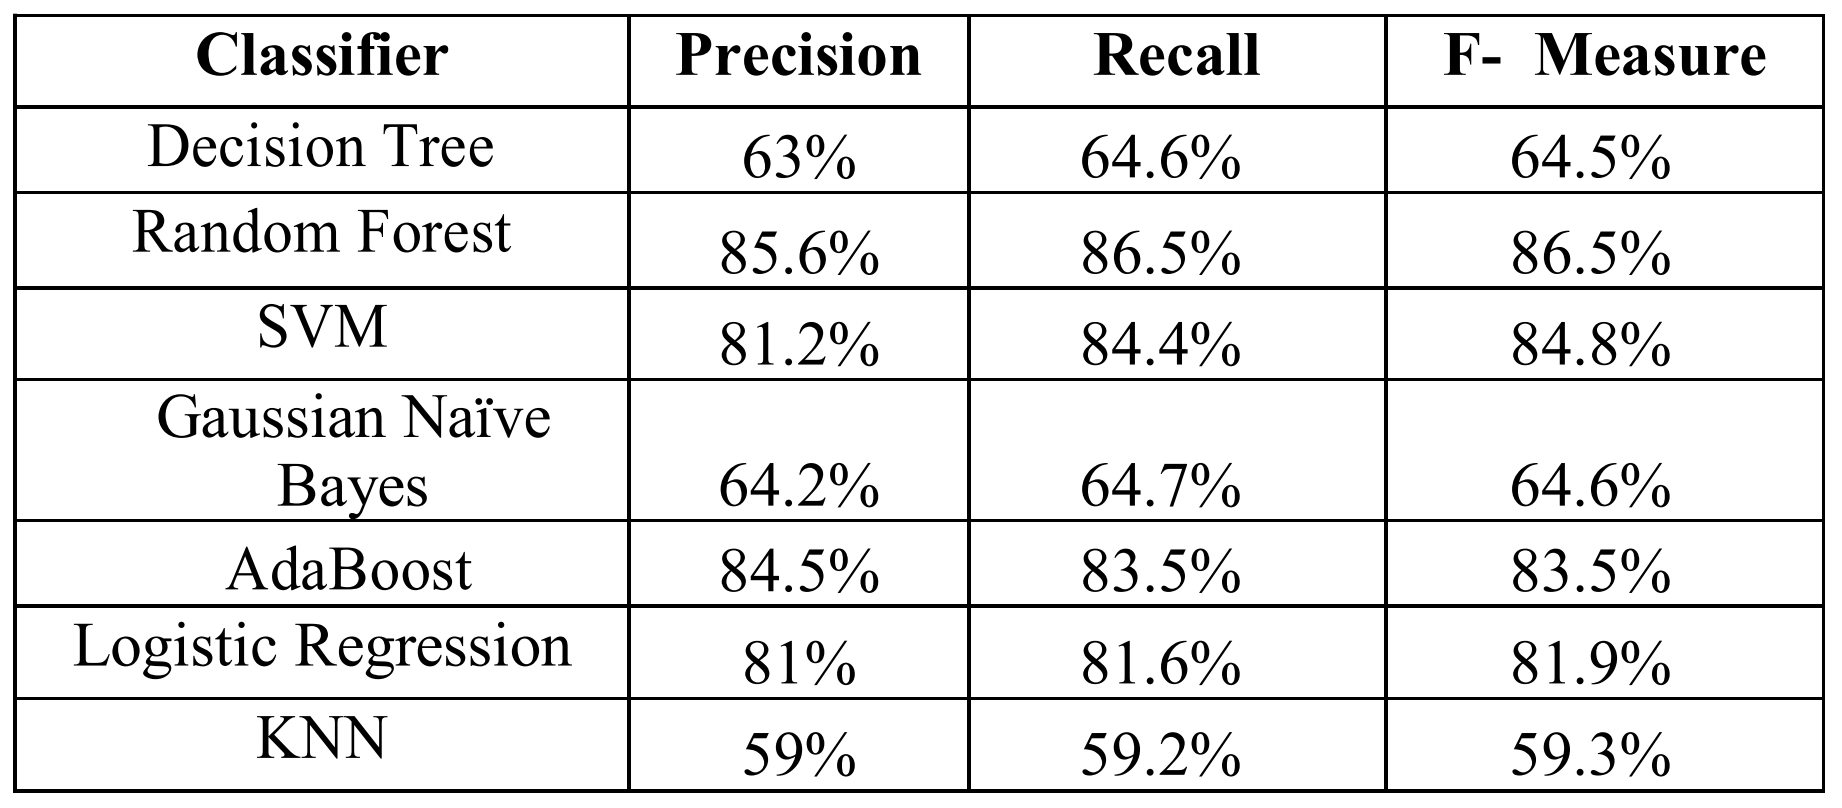
\includegraphics[width=0.9\textwidth]{literature_review/arane_classifier_results.PNG}
\caption{\label{fig:arane} Accuracy of Classifier Results from the study by A. Rane and A. Kumar \cite{Rane2018}.}
\end{figure}

\section{Sentiment Analysis}

Sentiment analysis is the process of identifying the opinion expressed about a particular subject in some text. The aim is to determine whether the opinion is positive, negative or neutral, and to what extent. Sentiment analysis makes use of natural language processing (NLP) and machine learning. This section will discuss the two main approaches to sentiment analysis, lexicon based approaches and supervised machine learning based approaches. 

A lexicon-based approach works by classifying a sentence based on the number of opinion words (positive or negative words) in the sentence. A sentiment score is calculated based on the ratio of positive to negative words. Unlike supervised machine learning methods, no training data is required. However, a lexicon is required and these are not available for every language. The lexicon approach has limitations, it does not allow for a term to be positive in one context but negative in another. It also cannot deal with an opinion being expressed towards multiple entities in a single sentence.

Supervised machine learning approaches require labelled training data. Their performance is very dependent on the size and quality of the set of training data. The accuracy of a classifier depends on the features selected for training and the domain the classifier is applied to. A method that performs well on a set of reviews from Tripadvisor will not necessarily perform well on a set of Tweets. Each method needs to be adapted to the specific domain it will be used on.

S. Bhuta, A. Doshi, U. Doshi, and M. Narvekar \cite{Bhuta2014} reviewed different methods for the sentiment analysis for text, with a focus on Twitter. These included a lexicon approach and three supervised learning methods, Naive Bayes, Maximum Entropy and Support Vector Machines. The three supervised learning methods generally outperform the lexicon-based approach. There are two first order probabilistic models for Naive Bayes, Bernoulli and Multinomial. Bernoulli performs better on smaller vocabularies and Multinomial performs better on larger vocabularies. The bigram Naive Bayes outperformed the unigram and ${X}^2$ feature selection improved its accuracy. Maximum Entropy, a probability distribution estimation technique, has an advantage over Naive Bayes as it does not suffer from the independence assumption. Maximum Entropy does suffer from over-fitting, which can be improved using maximum a posteriori estimation. Support Vector Machines can handle large feature spaces which is useful for Twitter data. A disadvantage of Support Vector Machines is that they are a black box method. It can be hard to know exactly what is having an effect on the algorithm and how to improve it.

\begin{figure}[h!]
\centering
\fbox{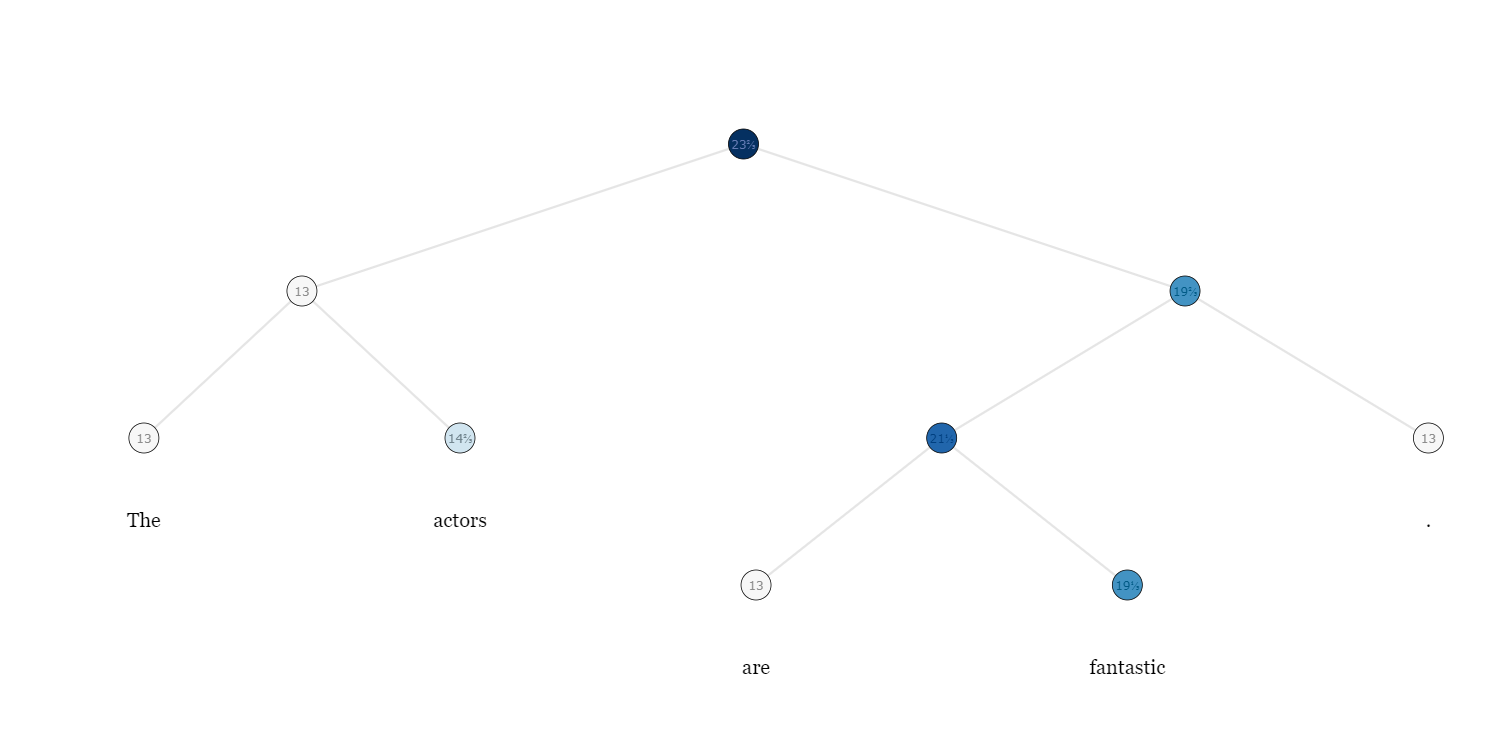
\includegraphics[width=0.9\textwidth]{literature_review/sample_treebank.PNG}}
\caption{\label{fig:treebank} A labelled movie review in the Stanford NLP Sentiment Treebank \cite{stanfordSentiment2013}.}
\end{figure}

The Stanford NLP (Natural Language Processing) Group's Sentiment Analyser \cite{stanfordSentiment2013} introduced a Recursive Neural Tensor Network (RNTN) along with a Sentiment Treebank. The Sentiment Treebank extended the corpus of movie reviews originally collected by Pang and Lee \cite{panglee2004}. The sentences in the movie review corpus were relabelled at a phrase level, producing a sentiment labelled parse-tree for each review (Figure ~\ref{fig:treebank}). The Sentiment Treebank produced has more finely grained sentiment labels than the original corpus. It improved how the compositional effects of sentiment in language were captured. For example, a word may be positive in one context but negative in another. In this sentence, 'The phone has a really long battery life', long is positive, however in this sentence, 'The website took so long to load', long is negative. All classification models trained with the Sentiment Treebank saw a significant increase in accuracy. These included Naive Bayes, Support Vector Machines, and other recursive neural networks. The RNTN achieved the highest accuracy of 85.4\% in single sentence positive/negative classification.

\section{Recommender Systems}

Recommender systems recommend items to users, based on what they predict is most likely to be of interest to the user. Their aim is to recommend the item best suited to the individual's preferences. Recommenders have been used in numerous areas such as film recommendations on Netflix, friend recommendations on Facebook, product recommendations on Amazon and hotel recommendations on TripAdvisor. They try to help consumers overcome information overload.

A number of recommender systems that focus on hotels have been proposed in the literature. A. Levi, O. Mokryn, C. Diot, and N. Taft proposed a recommender system that specifically focuses on hotel recommendations. A cold start, context-based hotel recommender system, which uses the text of online reviews from Tripadvisor and Venere as its main data \cite{levi2012}. The system asks the user to identify their trip intent (e.g. business, family etc), nationality and preferences for certain hotel aspects (location, service, food etc). Hotels are recommended based on the sentiment reviews of users who have similar context information.

Another recommender system that targets hotel was proposed by K. Lin, C. Lai, P. Chen, and S. Hwang \cite{lin2015}. It also uses hotel reviews collected from TripAdvisor. The system tracks the user's gestures on a mobile device to identify what part of the review the user has focused on or 'seriously read'. Feature extraction is used to extract the aspects of hotels (e.g room, food, price etc) the user considers important, and build a user interest profile. Hotels are recommended based on the user profile. The score is calculated based on the sentiment of the reviews about the aspects of the hotels the user prefers.

J. Chang, C. Tsai, and J. Chiang \cite{chang2018} proposed a hotel recommendation system that uses a combination of Twitter and Yelp data. They use a collaborative filtering method. The idea is that Twitter provides limited information on its own, but when combined with Yelp, which has explicit user ratings, can achieve better performance in a recommender system. User posting behaviour vectors are generated for both Twitter and Yelp and are combined to make recommendations.

Takehara, T. and Miki, S. and Nitta, N. and Babaguchi, N. propose a rule-based method of extracting context information from Twitter for use alongside a restaurant recommender system \cite{takeharaContext2012}. Relevant keywords are extracted from reviews from Tabelog \footnote{\url{https://tabelog.com}} (a Japanese review site) and are used to search Twitter for the contextual information. Nouns are extracted from Tabelog using part-of-speech tagging. Those characteristically used for assessing restaurants in each area are selected as keywords and categorised as area related keywords or restaurant related keywords. Finally, tweets containing more than two nouns from each set of keywords (area and restaurant) are selected as the contextual information and are displayed alongside the restaurant recommendations.
\chapter{Design and Methodology}

\section{Introduction}

In this chapter the design and methodology choices involved in this project will be presented. This project consists of five main stages (Figure ~\ref{fig:pipeline}), each of which will be discussed in this chapter. These five stages are:
\begin{itemize}
    \item Data Collection and Filtering: Collecting the twitter data and filtering it so it only contains tweets about hotels posted from Dublin.
    \item Dataset Annotation: Annotating the filtered dataset.
    \item Classification: Training and evaluating multiple supervised machine learning classifiers with different feature representations.
    \item Sentiment Analysis: Analysing the sentiment of those tweets classified as reviews.
    \item Application to Recommender System: Using the sentiment scores produced to re rank the results of the CoRE\cite{core2019} recommender system.
\end{itemize}

\begin{figure}[h!]
\centering
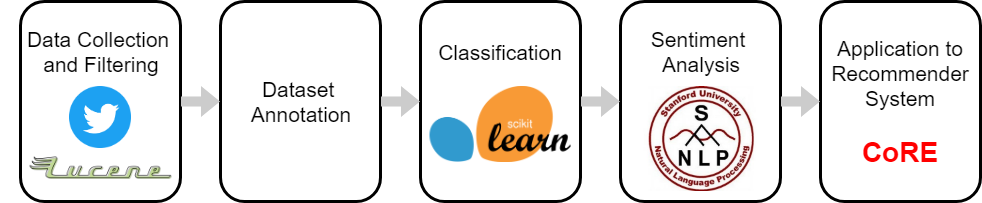
\includegraphics[width=1\textwidth]{design_and_methodology/pipeline.png}
\caption{\label{fig:pipeline} Overview of Project.}
\end{figure}

\section{Data Collection}
The data was collected using the Twitter Streaming API \footnote{\url{https://developer.twitter.com}} between October 2017 and September 2018. Twitter has a Search API and a Streaming API. The Search API allows you to find historical tweets and the Streaming API allows you to stream real-time tweets.

The data for this project was collected using the Streaming API. A filter was specified so that only tweets posted from within a bounding box of Dublin were returned. A total of 2.5 million tweets were collected.

After inspecting the collection of tweets it was found that although a bounding box had been specified not all tweets in the collection were posted from Dublin. A significant amount of tweets had slipped through Twitter's location filter. This meant the first step was to filter the dataset.

\section{Data Filtering}

\subsection*{Geo-tagged Tweets}

All of the tweets in the dataset were Geo-tagged since they were collected with a location filter. This meant they all had location data; a specified location from which the tweet was posted. There are two main types of Geo-tagged tweets:
\begin{itemize}
    \item Tweets with a specific latitude/longitude or 'Point' coordinate. These tweets come from GPS enabled devices (Listing ~\ref{lst:pointjson}).
    \item Tweets with a bounding box or Twitter 'Place'. A bounding box is a four-sided geographic area, defined by four points of the form [longitude, latitude] (Figure ~\ref{fig:dublinBB}). This defines the general area the tweet was posted from (Listing ~\ref{lst:placejson}).
\end{itemize}

\begin{figure}[h!]
\centering
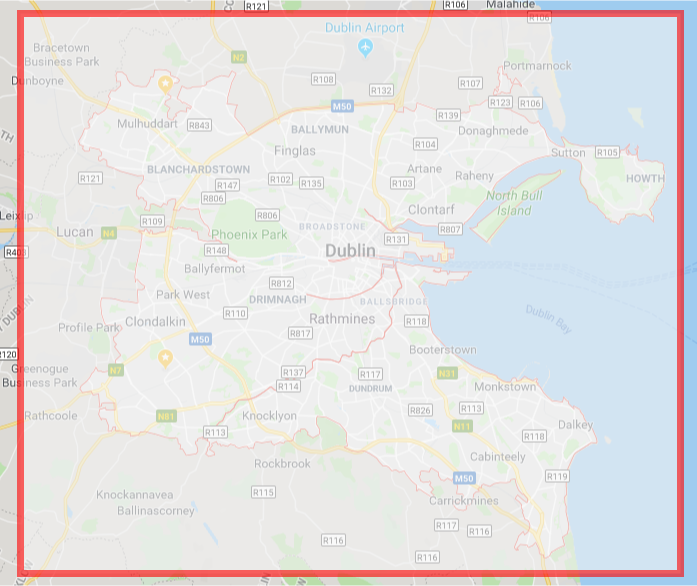
\includegraphics[width=0.6\textwidth]{design_and_methodology/dublinBB.png}
\caption{\label{fig:dublinBB} Bounding Box for Dublin.}
\end{figure}

\begin{lstlisting}[caption={Geo-tagged Tweet with Point Coordinate},
captionpos=b,label=lst:pointjson,language=json,firstnumber=1]
"geo": {
    "type": "Point",
    "coordinates": 
        53.28581863,
        -6.11439315
    ]
}
\end{lstlisting}

\begin{lstlisting}[caption={Geo-tagged Tweet with Twitter Place},captionpos=b,label=lst:placejson,language=json,firstnumber=1]
"place": {
  "full_name": "Dun Laoghaire-Rathdown, Ireland",
  "url": "https://api.twitter.com/1.1/geo/id/723427e351a01e72.json",
  "country": "Ireland",
  "place_type": "city",
  "bounding_box": {
    "type": "Polygon",
    "coordinates": [
      [
        [
          -6.282038,
          53.199283
        ],
        [
          -6.282038,
          53.315283
        ],
        [
          -6.066759,
          53.315283
        ],
        [
          -6.066759,
          53.199283
        ]
      ]
    ]
  },
  "country_code": "IE",
  "attributes": {},
  "id": "723427e351a01e72",
  "name": "Dun Laoghaire-Rathdown"
}
\end{lstlisting}

\subsection*{Filtering Out Non-Dublin Tweets}

The first attempt to filter out any non Dublin tweets involved using the point coordinate of the tweets. The point coordinate of each tweet was compared to the bounding box of Dublin. If it lay inside the box it was kept, otherwise it was filtered out. However, only 7.23\% of the tweets in our collection actually had a specific 'Point' coordinate. Filtering based on this excluded the majority of the dataset. To address this we instead filtered tweets based on either their point coordinate or their Twitter place.

All of the tweets in the collection have a Twitter place defining the general area that the tweet was posted from. A combination of the Twitter place and the point coordinates was used to filter out any non Dublin tweets that had ended up in the dataset. 

\begin{table}[h!]
\caption{Coordinates for Dublin's Bounding Box}
\label{tab:dublinbb}
\begin{tabular}{cc}
\hline
North Latitude  & 53.425210 \\ \hline
South Latitude  & 53.223430 \\ \hline
East Longitude & -6.043924 \\ \hline
West Longitude & -6.447485 \\ \hline
\end{tabular}
\end{table}

A bounding box for the Dublin area was defined (Table ~\ref{tab:dublinbb}). Tweets with a point coordinate and tweets with only a Twitter place were filtered differently:
\begin{itemize}
    \item \textbf{Point Coordinates}\newline
    Each tweet with a point coordinate was checked to see if it fell within the defined bounding box for Dublin. If it lay inside the box it was kept, otherwise it was filtered out.
    \item \textbf{Twitter Place}\newline
    Each tweet with a Twitter place has a bounding box specifying the location of the place. The centroid of this bounding box was calculated for each tweet. Then the centroid was checked to see if it fell within the defined bounding box for Dublin. If it lay inside the box it was kept, otherwise it was filtered out.
\end{itemize}

The filtered dataset consisted of 1.6 million tweets posted from Dublin between October 2017 and September 2018.

\subsection*{Filter Out Tweets About Hotels}

Now that the dataset had been filtered so that it only contained tweets posted from Dublin, the next step was to extract the tweets that mentioned hotels.

A list of the hotels in Dublin was compiled. This included the hotel's name and the hotel's Twitter handle (@hotelname). This list consisted of ?? hotels and Twitter handles.

The tweets were stored in a Lucene index. A fuzzy search query was used to match the tweets against each of the hotel names and hotel Twitter handles. The fuzzy search query uses a similarity measure that is based on the Damerau-Levenshtein algorithm. The maximum edits option was set to two. This means that strings with a maximum difference of two characters would match. This accounted for misspellings and broadened our search slightly. We experimented with higher numbers of maximum edits but found that too many irrelevant tweets were returned.

This further filtered dataset consisted of 3116 tweets that mention hotels posted from Dublin between October 2017 and September 2018.

\section{Dataset Annotation}

One major goal of this research was to categorise tweets as review-like tweets, tweets that contain some content and irrelevant tweets. In order to train a classifier to do this a set of tweets had to first be manually annotated. The set of 3116 tweets about hotels in Dublin was annotated. This involved building an annotation webpage where users could view tweets and assign them a label.

\subsection*{Annotation Webpage}

A simple webpage was created in order to annotate the tweets (Figure ~\ref{fig:webpage}). The webpage can be found at \url{http://reviewtweets.epizy.com}. The text of each tweet was displayed alongside three buttons; review, some content and irrelevant. The participant could click on the option they thought best described the tweet shown. Once they chose a label, the next tweet would be displayed. 

Each time the webpage is loaded a random tweet from the dataset is displayed. The participant can annotate the tweets incrementally from that random tweet on. This means each participant will label a different section of the tweets, ensuring all tweets in the collection get annotated evenly.

The following instructions, describing what a review, some content and irrelevant tweet should look like accompanied the webpage:
\begin{itemize}
    \item \textbf{Review} \newline
    The tweet could be considered as a review (of any aspects related to a hotel such as the venue, food, view, swimming pool etc.) for any hotel. Examples would include: \emph{"Amazing view of the Aviva Stadium from my hotel balcony at hotel X"} (positive review), "Room service was awful at hotel Y" (negative review), \emph{"Thank you hotel X for a lovely stay"} (positive review) or \emph{"Had an awful night at hotel Y"} (negative review).
    \item \textbf{Some Content} \newline
    The tweet doesn't look like a review, but it does provide some information related to a hotel, such as the hotel hosts events, information on the menu, information related to accommodation etc. Examples would include: \emph{"Hotel Z serves Tuna salad on Wednesday”} or \emph{“A packed room for the 2018 fashion conference at Hotel X”}.
    \item \textbf{Irrelevant} \newline
    This tweet is completely irrelevant. While perhaps mentioning the name of a hotel, the tweet doesn't give any additional information about that hotel or offer any opinions related to the hotel.
\end{itemize}

In this research we decided to focus solely on the text of the tweets. For this reason all images, videos and URLs were removed from the tweets.

\begin{figure}[h!]
\centering
\fbox{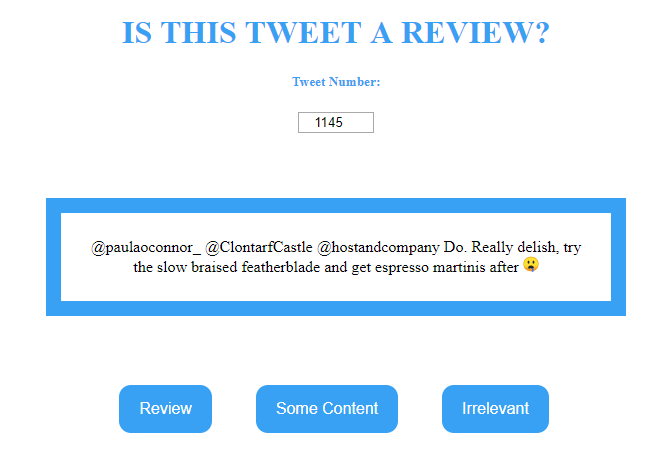
\includegraphics[width=1\textwidth]{design_and_methodology/webpage.PNG}}
\caption{\label{fig:webpage} Webpage for gathering Tweet Annotations.}
\end{figure}

The tweets were stored in an SQL table (Table ~\ref{Table:TweetAnnotation}) linked to the webpage, along with a count of the number of times the tweet had been labelled as a review, some content or irrelevant. Each time a participant chooses a label the corresponding value in the database is incremented. The final label of a tweet is determined by calculating which label had the maximum number of votes. 

\begin{table}[h!]
\caption{Sample of tweets from SQL table}
\label{Table:TweetAnnotation}
\setlength\extrarowheight{5pt}
\begin{tabular}{llllll}
\specialrule{1.5pt}{1pt}{1pt}
    \multicolumn{1}{l}{\textbf{Row No.}} & 
    \multicolumn{1}{l}{\textbf{Tweet ID}} & 
    \multicolumn{1}{l}{\textbf{Tweet}} & 
    \multicolumn{1}{l}{\textbf{Review}} & 
    \multicolumn{1}{l}{\textbf{Content}} & 
    \multicolumn{1}{l}{\textbf{Irrelevant}} \\ 
\specialrule{1.5pt}{1pt}{1pt}
\rowcolor[HTML]{EFEFEF} 
    1 & 00000 & 
    \begin{tabular}[c]{@{}l@{}}
        Creating A Rewarding Experience\\ 
        or CARE, essence of any\\ DoubleTree by Hilton hotels, \\ 
        is in the heart of everything in the\\ 
        Morrison Hotel! \#CARE \\
        \#DoubleTree \#dublincity \\ 
        \#brandculture
    \end{tabular} & 0 & 0 & 0 \\ 
\hline
    2 & 00000 & 
    \begin{tabular}[c]{@{}l@{}}
        @bfitzsimons @doubletree \\
        @DTHydePark Oohh. \\
        Impressed!
    \end{tabular} & 0 & 0 & 0 \\ 
\hline
\rowcolor[HTML]{EFEFEF} 
    3 & 00000 & 
    \begin{tabular}[c]{@{}l@{}}
        SlowMo Training \\ 
        \#EliteFest2018 @ The \\ 
        Morrison, a DoubleTree \\ 
        by Hilton Hotel
    \end{tabular} & 0 & 0 & 0 \\ 
\hline
    4 & 00000 & 
    \begin{tabular}[c]{@{}l@{}}
        Drinking a Heineken by \\ 
        @heineken at @doubletree —
    \end{tabular} & 0 & 0 & 0 \\ 
\hline
\end{tabular}
\end{table}

The annotation webpage was circulated to friends, family and members of the Adapt Research Centre to gather annotations.

\section{Tweet Classification}

The annotated set of tweets was used to train a series of different classifiers. These classifiers were implemented using Python's Scikit Learn library \cite{scikit-learn}. The data was split into a training set and a testing set. The data was split 80:20 where 80\% was used for training and 20\% was used for testing.

\subsection*{Data Preprocessing}

The following steps were taken to preprocess the tweets, before they were used to train the classifiers:
\begin{itemize}
    \item Emojis were removed and replaced with text using Python's Emoji library \cite{emoji}. For example a thumbs up emoji would be converted to the text \emph{':thumbs\_up:'} and then \emph{'thumbs up'} once punctuation is removed.
    \item Special characters and punctuation were removed. This included everything except the digits 0 - 9 and the letters a - z (upper and lower case).
    \item All single characters were removed.
    \item Words were split on case changes. For example \emph{'MerrionHotel'} --> \emph{'Merrion Hotel'}.
    \item Words were split on word-digit boundaries. For example \emph{'HouseDublin2'} --> \emph{'House Dublin 2'}.
    \item All text was converted to lower case.
    \item Stemming was performed using the Word Net Lemmatizer. Stemming is the process of reducing words down to their base or root. For example \emph{'organise'}, \emph{'organised'} and \emph{'organisation'} would all be reduced to \emph{'organis'}. Stemming conflates similar terms, reducing the number of words that are fed to the classifier.
    \item Stop words were removed. All text contain words that are irrelevant and do not add any additional meaning. These are called stop words. Some examples of stop words are \emph{'and'}, \emph{'I'}, \emph{'of'} and \emph{'the'}.
\end{itemize}

\subsection*{Feature Extraction}

The classifiers require numerical feature vectors of fixed length rather than variable length raw text as their input. To comply with this our processed tweets had to be converted into numerical feature vectors. This process of converting raw text to a numerical feature vector is called vectorization.

We experimented with six different feature extraction methods to see which performed best on the Twitter data. Twitter data is quite different to standard text so standard feature extraction methods that perform well on text will not necessarily perform well for the Twitter data.

The six feature extraction methods implemented were:
\begin{enumerate}
    \item Unigram Bag-of-Words with TF-IDF.
    \item Bigram Bag-of-Words with TF-IDF.
    \item Trigram Bag-of-Words with TF-IDF.
    \item Unigram Bag-of-Words with TF-IDF (with stop words removed).
    \item Word2Vec.
    \item Doc2Vec.
\end{enumerate}

\subsubsection{Bag-of-Words}

In Bag-of-Words (BOW) documents are described by word occurrences. A vocabulary is created of all unique terms in the dataset. The vocabulary is ranked by frequency of occurrence. The maximum size of the vocabulary can be specified, so only the top however many terms are kept. Each tweet is then represented as a feature vector consisting of ones and zeroes. One representing a terms occurrence and zero representing a terms lack of occurrence. A major drawback of BOW is that it does not take word ordering into account. This is why it is called 'bag' of words. You can imagine all the words have been thrown into a bag together.

The Count Vectorizer from Python's Scikit Learn was used to implement BOW. 

\subsubsection{TF-IDF}

BOW can be extended with TF-IDF (Term Frequency Inverse Document Frequency). Term frequency is the frequency of the word in the current document. Inverse Document Frequency takes into account how often the word occurs in the whole dataset. The idea is to balance how important a term is in a document versus how important it is in the entire collection. We are less interested in a very frequently occurring term like for example 'the' than some less frequently occurring words. The TF-IDF score is used to re-weight the count features produced by the Count Vectorizer.

\begin{tcolorbox}[title=TF-IDF]
\begin{center}
$TF-IDF = term\ frequency \times inverse\ document\ frequency$ 

$TF = \frac{Number\ of\ Term\ Occurrences\ in\ Document}{Number\ of\ Terms\ in\ Document}$

$IDF = \log \frac{1\ +\ n}{1\ +\ df(t)} + 1$

$n = Total\ number\ of\ documents\ in\ the\ dataset.$

$df(t) = Number\ of\ documents\ in\ the\ dataset\ containing\ term\ t.$
\end{center}
\end{tcolorbox}
The TF-IDF transformer from Python's Scikit Learn was used to implement TF-IDF.

% SCIKIT: very short texts are likely to have noisy tf–idf values while the binary occurrence info is more stable.

\subsubsection*{N-Grams}

Another extension of BOW is the use of N-grams. N-grams help to address the problem BOW has with discarding word ordering.

An N-gram is a sequence of N consecutive terms. For example the bi-grams of \emph{'Twitter as an Alternative Review Site'} are:
\begin{itemize}
    \item \emph{'Twitter as'}
    \item \emph{'as an'}
    \item \emph{'an Alternative'}
    \item \emph{'Alternative Review'}
    \item \emph{'Review Site'}
\end{itemize}


Combing bi-grams with BOW means that occurrences of pairs of consecutive words are counted instead of individual terms. Uni-grams, bi-grams and tri-grams were implemented.

\subsubsection{Word2Vec}

Word2Vec is another method for converting text into numerical feature vectors. It takes a large dataset as it's input and produces a vector space. Each word in the dataset is represented by a corresponding vector. It groups the vector of similar words together in the vector space. Cosine similarity, the cosine of the angle between two vectors, measures the similarity of vectors in the vector space. 

Gensim's implementation of Word2Vec \cite{gensim} and Google's pre-trained model was used. Google's model includes word vectors for three million words and phrases. It was trained with about 100 billion words from a Google News dataset. The word vectors of each word in a document are averaged to produce a feature vector for each document.
% Similar to BOW? doesn't perform any better really, also has no relationship between words.

\subsubsection*{Doc2Vec}

Doc2Vec takes the same idea as Word2Vec, but instead of words being represented by vectors, full documents are represented as vectors. This captures the relationship between words, which Word2Vec does not.

Gensim's implementation of Doc2Vec was again used. Unlike Word2Vec, we built our own Doc2Vec vocabulary based on the training data.

\subsection*{Classifiers}

Twelve different classifiers were implemented, each with their implementation from Python's Scikit Learn library \cite{scikit-learn}.

The twelve classifiers implemented were:
\begin{enumerate}
    \item Decision Tree Classifier.
    \item Random Forest Classifier.
    \item Multi Layer Perceptron Classifier.
    \item Support Vector Machine Classifier.
    \item Logistic Regression Classifier.
    \item K Nearest Neighbours Classifier.
    \item Gaussian Process Classifier.
    \item Adaboost Classifier.
    \item Gaussian Naive Bayes Classifier.
    \item Bernoulli Naive Bayes Classifier.
    \item Quadratic Discriminant Analysis Classifier.
    \item Linear Discriminant Analysis Classifier.
\end{enumerate}

\subsubsection*{Decision Tree}

The Decision Tree Classifiers is a simple classification algorithm that can be used for binary or multi-class classification. They learn simple decision rules based on the attributes of the training data. These decision rules form a tree structure (Figure ~\ref{fig:decisiontree}) which is used to predict the value of a target variable. The leaf nodes represent the class labels. When an unclassified document is received questions are asked until a leaf node is reached and the document is assigned that class.

\begin{figure}[h!]
\centering
\fbox{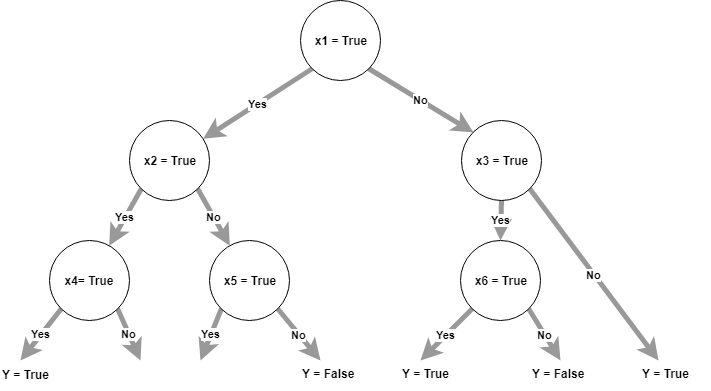
\includegraphics[width=0.75\textwidth]{design_and_methodology/decisiontree.png}}
\caption{\label{fig:decisiontree} Decision Tree Example}
\end{figure}

The DT Classifier was implemented with Scikit Learn with the following parameters:

\begin{tcolorbox}
\begin{center}
	DecisionTreeClassifier (criterion='entropy', max\_depth=32, max\_features=None, min\_samples\_leaf=2, min\_samples\_split=0.1)
\end{center}
\end{tcolorbox}

\subsubsection*{Random Forest}

%[B2001]	Breiman, “Random Forests”, Machine Learning, 45(1), 5-32, 2001.

The Random Forest Classifier (RF) is an ensemble classification algorithm, meaning it combines multiple base classification algorithms. It consists of multiple decision trees. The final class prediction is calculated by getting the average of the decision of the individual decision trees.

The RF Classifier was implemented with Scikit Learn with the following parameters:

\begin{tcolorbox}
\begin{center}
	RandomForestClassifier (n\_estimators=500, max\_features='log2', criterion='entropy')
\end{center}
\end{tcolorbox}

\subsubsection*{Multi Layer Perceptron}

The Multi Layer Perceptron (MLP) Classifier is a deep, feedforward, artificial neural network. It conists of a minimum of three layers (Figure ~\ref{fig:mlp}); an input layer, a hidden layer and an output layer. The input layer receives the data, the output layer makes a decision and the hidden layers approximate the function.

\begin{figure}[h!]
\centering
\fbox{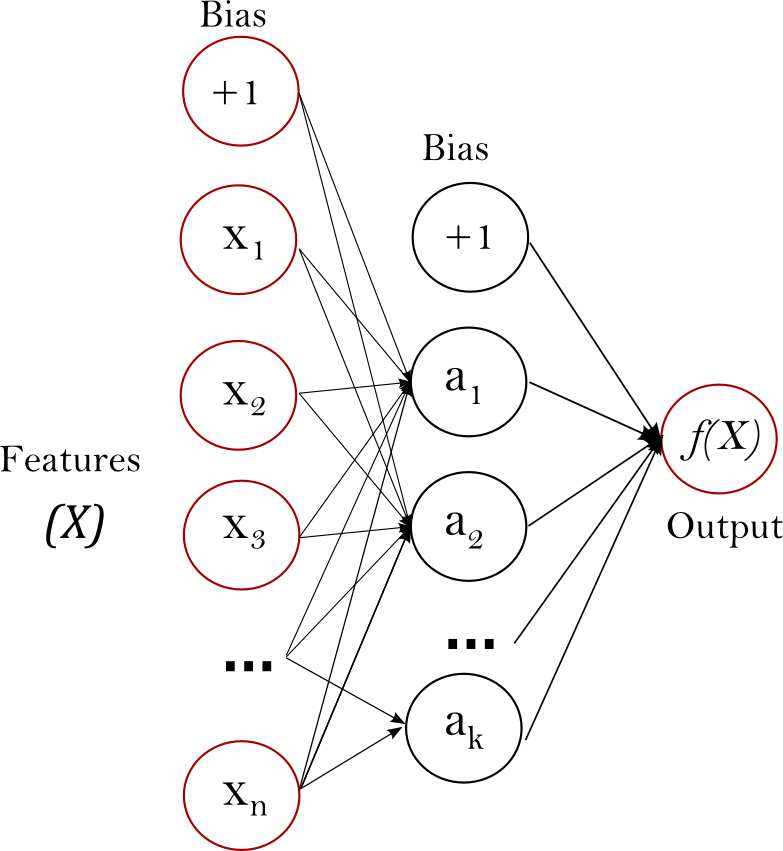
\includegraphics[width=0.5\textwidth]{design_and_methodology/multilayerperceptron_network.png}}
\caption{\label{fig:mlp} MLP with one hidden layer \cite{scikit-learn}}
\end{figure}

The MLP learns a function by based on the training set. Given a set of features X = x1,x2,x3,...,xn and a target y, it learns a non-linear approximation function. Backpropagation is used to train the MLP.

The MLP Classifier was implemented with Scikit Learn with the following parameters:

\begin{tcolorbox}
\begin{center}
	MLPClassifier (alpha=1,activation='identity', hidden\_layer\_sizes=(100,), learning\_rate='constant', solver='adam')
\end{center}
\end{tcolorbox}

\subsubsection*{Support Vector Machine}

The Support Vector Machine (SVM) Classifier is a discriminative classifier. It finds the optimum hyperplane that separates the data into the labelled classes. It aims to maximise the distance between the hyperplane and the support vectors (the points closest to the hyper plane).

\begin{figure}[h!]
\centering
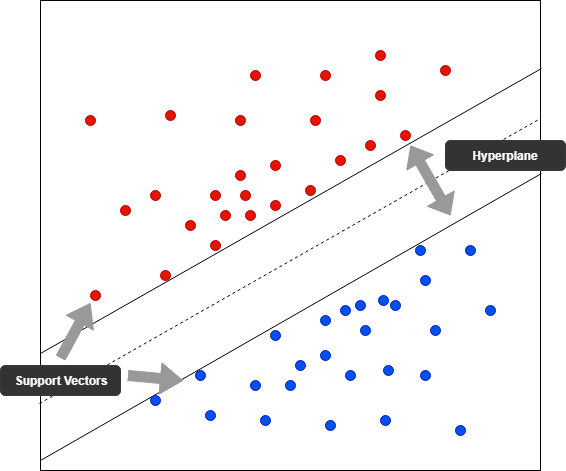
\includegraphics[width=0.75\textwidth]{design_and_methodology/svm.png}
\caption{\label{fig:svm} SVM.}
\end{figure}

The SVM Classifier was implemented with Scikit Learn with the following parameters:

\begin{tcolorbox}
\begin{center}
	SVC (C=10.1,decision\_function\_shape='ovo',degree=1,gamma=1,kernel='rbf')
\end{center}
\end{tcolorbox}

\subsubsection*{Logistic Regression}

The Linear Regression (LR) Classifier is a linear classification algorithm that uses the logistic function to model the training data. The logistic function is as follows:
\begin{center}
  \(g(z)=1/(1+e^{-z})\)  
\end{center}

The LR Classifier was implemented with Scikit Learn with the following parameters:

\begin{tcolorbox}
\begin{center}
	LogisticRegression (C=1,multi\_class='multinomial',penalty='l2',solver='saga')
\end{center}
\end{tcolorbox}

\subsubsection*{K Nearest Neighbours}

The K Nearest Neighbours (KNN) Classifier doesn't build a model like other classification algorithms. It uses a majority vote of the "nearest neighbours" to a document. A label is assigned to a document based on the class that has the majority of the nearest neighbours to the document. For example, point one would be assigned the label blue. Taking it's four nearest neighbours it has three blue neighbours and one red neighbour. The point is assigned to the class with the majority of the nearest neighbour, blue.

\begin{figure}[h!]
\centering
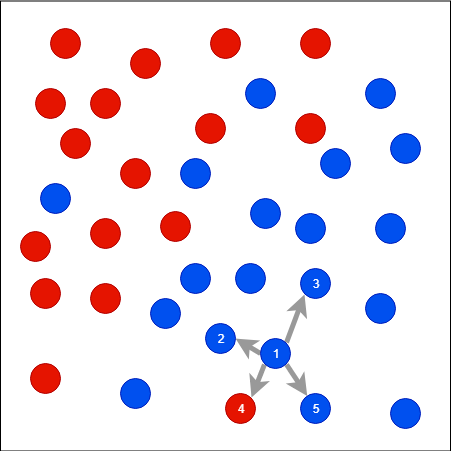
\includegraphics[width=0.7\textwidth]{design_and_methodology/knn.png}
\caption{\label{fig:knn} K Nearest Neighbours.}
\end{figure}

The KNN Classifier was implemented with Scikit Learn with the following parameters:

\begin{tcolorbox}
\begin{center}
	KNeighborsClassifier(n\_neighbors=17,algorithm='ball\_tree',weights='distance',
	leaf\_size=10,p=2)
\end{center}
\end{tcolorbox}

\subsubsection*{Gaussian Process}

The Gaussian Process (GP) Classifier implements Gaussian Processes for classification. Gaussian processes are probability distributions over possible functions.

The definition of a Gaussian process is: $P(f)$ is a Gaussian process if for any finite subset $\{x_1,x_2,...,x_n\} \subset X$, the marginal distribution over that finite subset $P(f)$ has a multivariate Gaussian distribution.

The GP Classifier puts a Gaussian process on a latent function, which is then squashed through a link function to get the probabilistic classification. For classification, the posterior of the latent function is not Gaussian, instead the logit function is used. A Gaussian likelihood function is inappropriate for discrete class labels \cite{gaussianProcesses2006}.

The GP Classifier was implemented with Scikit Learn with the following parameters:

\begin{tcolorbox}
\begin{center}
	GaussianProcessClassifier(kernel=1.0 * RBF(1.0), optimizer='fmin\_l\_bfgs\_b')
\end{center}
\end{tcolorbox}

\subsubsection*{Adaboost}

The AdaBoost Classifier is another ensemble classification algorithm, introduced by Freund and Schapire \cite{adaboost1997}.

AdaBoost works by fitting a series of weak base classifiers on incrementally re-weighted versions of the training data. The predictions from the base classifiers are combined with a majority vote or sum, to get an overall classification. The 'boosting' component of the algorithm involves re-weighting the data on each iteration.Samples that were predicted correctly have their weight increased and samples that were predicted incorrectly have their weight decreased.

The AdaBoost Classifier was implemented with Scikit Learn with the following parameters:

\begin{tcolorbox}
\begin{center}
	AdaBoostClassifier(base\_estimator=None, n\_estimators=50,learning\_rate=1, algorithm=’SAMME.R’)
\end{center}
\end{tcolorbox}

Scikit Learn's version of AdaBoost implements the SAMME algorithm \cite{multiclassada2009}.

\subsubsection*{Gaussian Naive Bayes}

The Gaussian Naive Bayes (GNB) Classifier is one of a set of Naive Bayes Classification algorithms. All of the Naive Bayes classifiers are based applying Bayes Rule along with the ‘naive’ assumption that features are conditionally independent. Bayes Rule: 
\begin{center}
\(P(A\mid B)=\frac{P(B\mid A)\:P(A)}{P(B)}\). 
\end{center}
In GNB the likelihood of the features is assumed to be Gaussian:
\begin{center}
$P(x_i|y) = \frac{1}{\sqrt{2\pi\sigma_y^2}} exp (- \frac{(x_i - \mu_y)^2}{2\sigma_y^2})$
\end{center}
The GNB Classifier was implemented with Scikit Learn with the following parameters:

\begin{tcolorbox}
\begin{center}
	GaussianNB (priors=None, var\_smoothing=1e-09)
\end{center}
\end{tcolorbox}

\subsubsection*{Bernoulli Naive Bayes}

The Bernoulli Naive Bayes (BNB) Classifier is another of the Naive Bayes Classification algorithms. BNB implements the Naive Bayes algorithm for data that is distributed according to multivariate Bernoulli distributions. It has been seen to work better than GNB on shorter texts.

The decision rule for BNB is:
\begin{center}
$P(x_i|y) = P(i|y)x_i + (1 - P(i|y))(1 - x_i)$
\end{center}

The BNB Classifier was implemented with Scikit Learn with the following parameters:

\begin{tcolorbox}
\begin{center}
	BernoulliNB (alpha=1.0, binarize=0.0, class\_prior=None, fit\_prior=True)
\end{center}
\end{tcolorbox}

\subsubsection*{Quadratic Discriminant Analysis and Linear Discriminant Analysis}

The Quadratic Discriminant Analysis Classifier and the Linear Discriminant Analysis Classifier, have a quadratic and linear decision surface, respectively. QDA is more flexible as it can learn quadratic boundaries, LDA can only learn linear boundaries (Figure ~\ref{fig:qdalda}). 

\begin{figure}[h!]
\centering
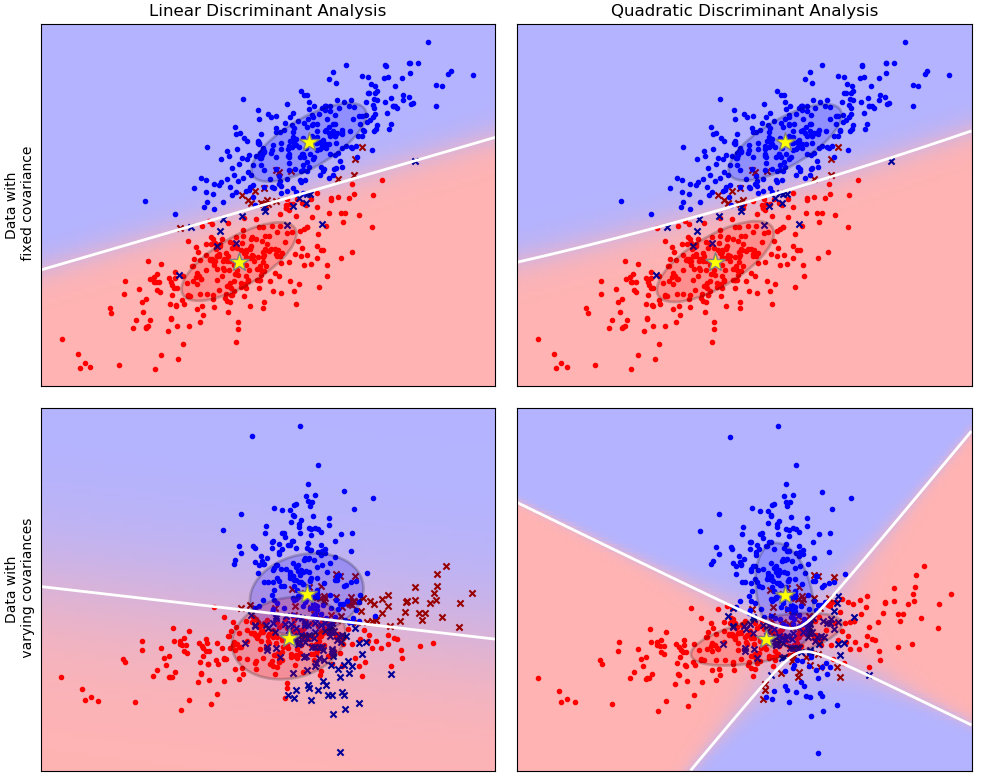
\includegraphics[width=1\textwidth]{design_and_methodology/qda_and_lda.png}
\caption{\label{fig:qdalda} Quadratic Discriminant Analysis and Linear Discriminant Analysis.}
\end{figure}

Both QDA AND LDA were implemented with Scikit Learn with the folllowing parameters:

\begin{tcolorbox}
\begin{center}
	QuadraticDiscriminantAnalysis(priors=None, reg\_param=0.0, store\_covariance=False, store\_covariances=None, tol=0.0001)
\end{center}
\end{tcolorbox}

\begin{tcolorbox}
\begin{center}
	LinearDiscriminantAnalysis(n\_components=None, priors=None, shrinkage=None, solver='svd', store\_covariance=False, tol=0.0001)
\end{center}
\end{tcolorbox}


\section{Sentiment Analysis}

Once the tweets had been classified as reviews, sentiment analysis was performed on them. Sentiment analysis is the process of identifying the opinion expressed about a particular subject in some text. The goal is to determine whether the opinion is positive, negative or neutral, and to what extent. The Stanford NLP Sentiment Analyser \cite{stanfordSentiment2013} was used to classify the sentiment of the tweets.

\subsection*{The Stanford Sentiment Analyser}

The Stanford Sentiment Analyser is based on a Recursive Neural Network. It was trained on a sentiment treebank of movie reviews from the movie review site RottenTomatoes. The treebank consists of sentences which are annotated on a phrase level. The Sentiment Analyser has reported accuracy of 85.4\% in single sentence positive/negative classification. 

The Stanford NLP Sentiment Analyser has it's limitations. Due to the fact that it was trained on movie reviews and is being applied to tweets, optimum performance is not achieved. Ideally the Sentiment Analyser would be re-trained with a set of tweets. This would involve manually annotating a collection of tweets at a phrase level to produce a treebank.

% we don't have pos/neg labels on the tweets so can't evaluate it's performance except for by eye?

The Stanford NLP Sentiment Analyser classifies the text into one of the following five sentiment judgements: 
\begin{enumerate}
    \item Very Negative
    \item Negative
    \item Neutral
    \item Positive
    \item Very Positive
\end{enumerate}

The output from the Sentiment Analyser for a tweet looks like this:

\begin{lstlisting}[caption={Output from Stanford NLP Sentiment Analyser},
captionpos=b,label=lst:stanfordoutput,language=json,firstnumber=1]
"sentimentValue": "3",
"sentiment": "Positive",
"sentimentDistribution": [
    0.03910365552553,
    0.18375415309071,
    0.26346977003905,
    0.42548434014862,
    0.0881880811961
]
\end{lstlisting}

The sentiment value and sentiment define the class the tweet has been assigned. In this case the tweet is positive. The sentiment distribution shows how strongly the tweet aligns with each class, from very negative to very positive. This tweet has a maximum value of 0.42548434014862 so it is assigned the positive label.

\subsection*{Normalisation}

The sentiment scores produced by the Stanford NLP Sentiment Analyser were produced per tweet. They needed to be normalised so that they were per hotel and lay between zero and one.

A majority voting technique was used to normalise the scores. For each hotel we have a selection of tweets. These tweets are divided into five clusters; very negative, negative, neutral (ignored), positive and very positive. A mean value was calculated for each cluster. This was calculated bu summing the corresponding score in the sentiment distribution for each tweet and dividing by the number of tweets in the cluster. The class with the highest mean value was assigned to the hotel.

This mean score was then normalised between zero and one, with the following weighting.
\begin{itemize}
    \item Very Negative: 0 --> 0.25
    \item Negative: 0.25 --> 0.5
    \item Positive: 0.5 --> 0.75
    \item Very Positive: 0.75 --> 1
\end{itemize}

The following normalisation formulae were used:

\begin{tcolorbox}
\begin{center}
	$Normalised\ Score\ (Negative) = max\ score\ -\ (actual\ score\ \times\ (max\ score\ -\ min\ score))$

    $Normalised\ score\ (Positive) = (actual\ score\ \times\ (max\ score\ -\ min\ score)) + min\ score$
\end{center}
\end{tcolorbox}

Taking the tweet above with a positive score of 0.42548434014862 as an example:
\begin{tcolorbox}
$Normalised\ score\ (Positive) = (0.42548434014862\ \times\ (0.75\ -\ 0.5)) + 0.5.$

$Normalised\ score\ (Positive) = 0.606$
\end{tcolorbox}

\section{CoRE Recommender System}

The sentiment scores produced by the Stanford Sentiment Analyser were used to re rank the list of hotel recommendations produced by the CoRE recommender system.

\subsection*{CoRE}
What core is...
\subsection*{Re-Ranking}
How CoRE was re-ranked...




\chapter{Evaluation}

\section{Introduction}
This chapter will present the results of this research. First, the evaluation metrics that were used to evaluate the classifiers will be introduced. The results of the evaluation of the thirteen classifiers with the seven different feature representations will be outlined. The methods used to evaluate the recommender system will be defined. Finally, the results of this evaluation will be presented. 

\section{Evaluation Metrics for Classification}

\subsection{Confusion Matrix}
A confusion matrix is a technique commonly used for evaluating the performance of a classification model. It presents a summary of the prediction results of the classifier. A confusion matrix consists of four different combinations of the actual values versus the predicted values (Table ~\ref{Table:confusionmatrix}). 

\begin{table}[h!]
\setlength\extrarowheight{5pt}
\caption{Confusion Matrix.}
\label{Table:confusionmatrix}
\begin{tabular}{c|c|c|}
\cline{2-3}
 & \multicolumn{1}{l|}{Actual Positive} & \multicolumn{1}{l|}{Actual Negative} \\ \hline
\multicolumn{1}{|l|}{Predicted Positive} & TP & FP \\ \hline
\multicolumn{1}{|l|}{Predicted Negative} & FN & TN \\ \hline
\end{tabular}
\end{table}

The values in a confusion matrix are:
\begin{itemize}
    \item \textbf{True Positive (TP)}\newline
    You have a True Positive value if your algorithm classified an item as positive and this was correct.
    \item \textbf{False Positive (FP)}\newline
    You have a False Positive value if your algorithm classified an item as positive but the value was actually negative.
    \item \textbf{False Negative (FN)}\newline
    You have a False Negative value if your algorithm classified an item as negative but the value was actually positive.
    \item \textbf{True Negative (TN)}\newline
    You have a True Negative value if your algorithm classified an item as negative and this was correct.
\end{itemize}

The confusion matrix is useful for calculating the precision, recall, accuracy and f1-score of a classification algorithm. These four metrics were used to evaluate the performance of the classifiers.

\subsection{Precision}
Precision is the percentage of positive identifications that were classified correctly.
\begin{equation}
    Precision\ =\ \cfrac{True\ Positives}{True\ Positives\ +\ False\ Positives}
\end{equation}
The higher the precision score the better. A low precision score can indicate that there is a large number of false positives. A high precision score indicates that the majority of what was classified, was classified correctly. You could however, have a very high precision score in the case where only a small portion of samples were actually classified but of these the majority were classified correctly. In this case the precision score is high but the recall would be very low.

\subsection{Recall}
Recall is the percentage of all actual positives that were classified correctly.
\begin{equation}
    Recall\ =\ \cfrac{True\ Positives}{True\ Positives\ +\ False\ Negatives}
\end{equation}
The higher the recall score the better. A low recall value can indicate that there are a large number of false negatives. A high recall value indicates that the majority of what should have been classified was classified correctly. You could however have a very high recall and low precision if everything was classified. All the samples that should have been classified are classified correctly, giving the high recall. But a lot of extra samples are classified that shouldn't have been classified, giving a low precision.

\subsection{Accuracy}
Accuracy is the total number of predictions the classifier got right. It is the percentage of the tweets that were classified correctly.
\begin{equation}
    Accuracy\ =\ \cfrac{Number\ of\ Correct\ Predictions}{Total\ Number\ of\ Predictions}
\end{equation}
The higher the accuracy score the better, but a high accuracy does not always give an accurate representation of the situation if there is a major class imbalance.

\subsection{F1-Score}
F1-Score is the harmonic mean of precision and recall. It is also called the F-Score or F-Measure. 
\begin{equation}
    F1-Score\ =\ 2 \times\ \cfrac{Precision\ \times\ Recall}{Precision\ +\ Recall}
\end{equation}
The higher the F1-Score the better. A high F1-Score indicates a good balance between precision and recall.

\subsection{Multi-Class Classification}
Multi-Class Classification is any classification task that involves two or more classes. This research tackles a multi-class classification problem. We aim to classifying tweets as one of the following three classes: 'Review', 'Some Content', or 'Irrelevant'. For a binary classification problem, the precision, recall, f1-score and accuracy scores can be calculated simply with the above formulas. For multi-class classification there needs to be a way of getting an average metric over the three classes, rather than an individual class score.
There are three ways that precision, recall, f1-score and accuracy can be calculated for this kind of multi-class classification problem:
\begin{enumerate}
    \item \textbf{Micro Average:}\newline
    The micro average calculates the metrics globally. It aggregates the contributions of all classes, counting the total true positives, false negatives and false positives, to calculate the overall average scores.  
    \item \textbf{Macro Average:}\newline
    The macro average calculates the metrics independently for each class. It then calculates the unweighted mean of the scores of the three classes.
    \item \textbf{Weighted Average:}\newline
    The weighted average calculates the metrics independently for each class, like the macro average does. It then calculates the weighted average of the scores of the three classes. This differs from the macro average in that it takes class imbalance into account. Class imbalance means that there is a significant amount more or less samples in one class. In our case there are significantly more tweets labelled as irrelevant than there are labelled as reviews (Table ~\ref{Table:tweetlabels}).
\end{enumerate}

The metrics listed in the tables below (Tables ~\ref{Table:precision},~\ref{Table:recall},~\ref{Table:accuracy},~\ref{Table:f1score}) were calculated with the weighted average.

\section{Classification Results and Analysis}

In this section, the results and evaluation of the classifiers will be presented. The classifiers evaluated include:
\begin{enumerate}
    \item Random Forest (RF) Classifier.
    \item Decision Tree (DT) Classifier.
    \item Multi Layer Perceptron (MLP) Classifier.
    \item Logistic Regression (LR) Classifier.    
    \item Support Vector Machine (SVM) Classifier.
    \item K Nearest Neighbours (KNN) Classifier.
    \item Gaussian Process (GP) Classifier.
    \item AdaBoost (AB) Classifier.
    \item Gaussian Naïve Bayes (GNB) Classifier.
    \item Multinomial Naïve Bayes (MNB) Classifier.
    \item Bernouilli Naïve Bayes (BNB) Classifier.
    \item Quadratic Discriminant Analysis (QDA) Classifier.
    \item Linear Discriminant Analysis (LDA) Classifier.
\end{enumerate}

These classifiers were evaluated with seven different feature representations defined below:
\begin{enumerate}
    \item Unigram BOW.
    \item Unigram TF-IDF.
    \item Bigram TF-IDF.
    \item Trigram TF-IDF.
    \item Unigram TF-IDF with stop words removed.
    \item Word2Vec.
    \item Doc2Vec.
\end{enumerate}

Taking the thirteen classifiers and seven feature representations there are 91 different combinations. Each was evaluated in terms of precision, recall, accuracy and f1-score.

The set of 3115 tweets was divided into a training set and a testing set with a 80:20 split. The label distribution of the data is shown in the table below (Table ~\ref{Table:tweetlabels}).

\begin{table}[h!]
\setlength\extrarowheight{5pt}
\caption{Distribution of Tweet Labels.}
\label{Table:tweetlabels}
\begin{tabular}{|c|c|}
\hline
\textbf{Label} & \textbf{Tweet Count} \\ \hline
Review         & 566                  \\ \hline
Some Content   & 910                  \\ \hline
Irrelevant     & 1639                 \\ \hline
\end{tabular}
\end{table}

\subsection{Precision}

In terms of precision, the QDA Classifier with unigram TF-IDF and no stop words feature representation was the best performing classifier achieving a precision score of 0.79 (Table ~\ref{Table:precision}). This indicates that the QDA Classifier had a high percentage of positive identifications that were classified correctly. The QDA Classifier with unigram TF-IDF feature representation, this time with stop words included achieved the next highest precision score of 0.76. This further confirmed that unigram feature representation seems to work best with the QDA Classifier. The RF Classifier and the SVM Classifier, both with unigram TF-IDF feature representations were the two next best performing classifiers both achieving precision values of 0.74.

\begin{table}[h!]
\setlength\extrarowheight{5pt}
\caption{Precision of Classifiers for different Feature Representations.}
\label{Table:precision}
\resizebox{\textwidth}{!}{
\begin{tabular}{cccccccc}
\specialrule{1.5pt}{1pt}{1pt}
 & \textbf{BOW} & \textbf{\begin{tabular}[c]{@{}c@{}}TF-IDF\\ (Unigram)\end{tabular}} & \textbf{\begin{tabular}[c]{@{}c@{}}TF-IDF\\ (Bigram)\end{tabular}} & \textbf{\begin{tabular}[c]{@{}c@{}}TF-IDF\\ (Trigram)\end{tabular}} & \textbf{\begin{tabular}[c]{@{}c@{}}TF-IDF\\ (Unigram,\\ No Stop Words)\end{tabular}} & \textbf{Word2Vec} & \textbf{Doc2Vec} \\ \specialrule{1.5pt}{1pt}{1pt}
\textbf{RF} & 0.72 & 0.74 & 0.7 & 0.69 & 0.73 & 0.71 & 0.59  \\ \hline
\rowcolor[HTML]{EFEFEF} 
\textbf{DT} & 0.57 & 0.58 & 0.58 & 0.59 & 0.63 & 0.54 & 0.56  \\ \hline
\textbf{MLP} & 0.71 & 0.71 & 0.7 & 0.7 & 0.7 & 0.71 & 0.59  \\ \hline
\rowcolor[HTML]{EFEFEF} 
\textbf{SVM} & 0.56 & 0.74 & 0.73 & 0.71 & 0.71 & 0.71 & 0.62  \\ \hline
\textbf{LR} & 0.72 & 0.72 & 0.7 & 0.68 & 0.7 & 0.71 & 0.61  \\ \hline
\rowcolor[HTML]{EFEFEF} 
\textbf{KNN} & 0.53 & 0.62 & 0.62 & 0.62 & 0.61 & 0.67 & 0.54  \\ \hline
\textbf{GP} & 0.72 & 0.72 & 0.71 & 0.69 & 0.7 & 0.72 & 0.61  \\ \hline
\rowcolor[HTML]{EFEFEF} 
\textbf{AB} & 0.63 & 0.62 & 0.63 & 0.62 & 0.64 & 0.63 & 0.57  \\ \hline
\textbf{GNB} & 0.6 & 0.6 & 0.63 & 0.63 & 0.59 & 0.64 & 0.59  \\ \hline
\rowcolor[HTML]{EFEFEF} 
\textbf{MNB} & \multicolumn{1}{c}{\cellcolor[HTML]{EFEFEF}0.71} & 0.67 & 0.68 & 0.66 & 0.67 & 0.32 & 0.35    \\ \hline
\rowcolor[HTML]{FFFFFF} 
\textbf{BNB} & 0.73 & 0.73 & 0.71 & 0.71 & 0.72 & 0.65 & 0.58  \\ \hline
\rowcolor[HTML]{EFEFEF} 
\textbf{QDA} & 0.72 & 0.76 & 0.73 & 0.67 & \textcolor{red}{0.79} & 0.59 & 0.57  \\ \hline
\rowcolor[HTML]{FFFFFF} 
\textbf{LDA} & 0.63 & 0.64 & 0.65 & 0.63 & 0.62 & 0.69 & 0.66  \\ \hline
\end{tabular}}
\end{table}

It is interesting to compare our precision scores to those in the study by A.Rane and A.Kumar \cite{Rane2018}, in which they investigated the performance of various classifiers in classifying the sentiment of Twitter reviews about airlines. They found that the RF Classifier achieved the highest precision score, followed first by the AdaBoost Classifier and then the SVM Classifier. They did not include the QDA Classifier in their evaluation. Our results do not fully confirm or contradict the results of A.Rane and A.Kumar \cite{Rane2018}. Two out of three of our top performing classifiers agree, the RF classifier and the SVM classifier. Their precision scores are higher than ours for all the classifiers that they implemented, at approximately 0.8 compared to ours at approximately 0.7. A likely reason for this is that they trained their classifiers on a much larger dataset, a total of 14640 tweets, while our classifiers were trained on a smaller set of 3116 tweets. Supervised machine learning methods tend to perform the best on large datasets. Our results could possibly be improved by collecting and annotating a larger dataset.

\subsection{Recall}

\begin{table}[h!]
\setlength\extrarowheight{5pt}
\caption{Recall of Classifiers for different Feature Representations.}
\label{Table:recall}
\resizebox{\textwidth}{!}{
\begin{tabular}{cccccccc}
\specialrule{1.5pt}{1pt}{1pt}
 & \textbf{BOW} & \textbf{\begin{tabular}[c]{@{}c@{}}TF-IDF\\ (Unigram)\end{tabular}} & \textbf{\begin{tabular}[c]{@{}c@{}}TF-IDF\\ (Bigram)\end{tabular}} & \textbf{\begin{tabular}[c]{@{}c@{}}TF-IDF\\ (Trigram)\end{tabular}} & \textbf{\begin{tabular}[c]{@{}c@{}}TF-IDF\\ (Unigram,\\ No Stop Words)\end{tabular}} & \textbf{Word2Vec} & \textbf{Doc2Vec} \\ \specialrule{1.5pt}{1pt}{1pt}
\textbf{RF} & 0.7 & 0.71 & 0.7 & 0.69 & 0.72 & 0.69 & 0.64  \\ \hline
\rowcolor[HTML]{EFEFEF} 
\textbf{DT} & 0.61 & 0.6 & 0.61 & 0.62 & 0.65 & 0.56 & 0.59  \\ \hline
\textbf{MLP} & 0.72 & 0.72 & 0.71 & 0.71 & 0.71 & 0.72 & 0.62  \\ \hline
\rowcolor[HTML]{EFEFEF} 
\textbf{SVM} & 0.59 & \textcolor{red}{0.74} & \textcolor{red}{0.74} & 0.72 & 0.72 & 0.72 & 0.64  \\ \hline
\textbf{LR} & 0.72 & 0.72 & 0.71 & 0.7 & 0.71 & 0.72 & 0.64  \\ \hline
\rowcolor[HTML]{EFEFEF} 
\textbf{KNN} & 0.61 & 0.66 & 0.66 & 0.65 & 0.65 & 0.68 & 0.61  \\ \hline
\textbf{GP} & 0.73 & 0.73 & 0.72 & 0.71 & 0.71 & 0.73 & 0.64  \\ \hline
\rowcolor[HTML]{EFEFEF} 
\textbf{AB} & 0.65 & 0.64 & 0.65 & 0.65 & 0.66 & 0.64 & 0.61  \\ \hline
\textbf{GNB} & 0.48 & 0.48 & 0.47 & 0.45 & 0.48 & 0.56 & 0.49  \\ \hline
\rowcolor[HTML]{EFEFEF} 
\textbf{MNB} & \multicolumn{1}{c}{\cellcolor[HTML]{EFEFEF}0.66} & 0.68 & 0.69 & 0.67 & 0.68 & 0.57 & 0.59  \\ \hline
\rowcolor[HTML]{FFFFFF} 
\textbf{BNB} & 0.71 & 0.71 & 0.66 & 0.62 & 0.71 & 0.56 & 0.54  \\ \hline
\rowcolor[HTML]{EFEFEF} 
\textbf{QDA} & 0.26 & 0.23 & 0.24 & 0.56 & 0.26 & 0.61 & 0.68  \\ \hline
\rowcolor[HTML]{FFFFFF} 
\textbf{LDA} & 0.61 & 0.61 & 0.61 & 0.59 & 0.59 & 0.69 & 0.67  \\ \hline
\end{tabular}}
\end{table}

The SVM Classifier was the best performing classifier with regard to recall, achieving a recall score of 0.74 (Table ~\ref{Table:recall}). The unigram TF-IDF and bigram TF-IDF feature representations performed equally well. This again partly agrees with A.Rane and A.Kumar \cite{Rane2018}, who found that the SVM Classifier was their second best performing classifier in terms of recall, with the RF classifier again coming out on top. Our scores are again slightly lower than those of A.Rane and A.Kumar \cite{Rane2018}.

Notice that the QDA Classifier which performed the best in precision, performs pretty poorly in terms of recall. This is a common issue and is why we have also evaluated the classifiers with the f1-score. The f1-score conveys the balance between precision and recall giving us a better idea of the actual performance of the classifier.

The GP Classifier was the next highest performing classifier, achieving a recall score of 0.73, with unigram TF-IDF feature representation. This is interesting as I have not come across any studies where a GP Classifier performs well in classifying tweets. The GP Classifier also performed well in precision achieving a precision score of 0.72.  

\subsection{F1-Score}

\begin{table}[h!]
\setlength\extrarowheight{5pt}
\caption{F1-Score of Classifiers for different Feature Representations.}
\label{Table:f1score}
\resizebox{\textwidth}{!}{
\begin{tabular}{cccccccc}
\specialrule{1.5pt}{1pt}{1pt}
 & \textbf{BOW} & \textbf{\begin{tabular}[c]{@{}c@{}}TF-IDF\\ (Unigram)\end{tabular}} & \textbf{\begin{tabular}[c]{@{}c@{}}TF-IDF\\ (Bigram)\end{tabular}} & \textbf{\begin{tabular}[c]{@{}c@{}}TF-IDF\\ (Trigram)\end{tabular}} & \textbf{\begin{tabular}[c]{@{}c@{}}TF-IDF\\ (Unigram,\\ No Stop Words)\end{tabular}} & \textbf{Word2Vec} & \textbf{Doc2Vec} \\ \specialrule{1.5pt}{1pt}{1pt}
\textbf{RF} & 0.65 & 0.65 & 0.64 & 0.64 & 0.69 & 0.63 & 0.59  \\ \hline
\rowcolor[HTML]{EFEFEF} 
\textbf{DT} & 0.57 & 0.59 & 0.58 & 0.6 & 0.63 & 0.54 & 0.56  \\ \hline
\textbf{MLP} & 0.71 & 0.7 & 0.69 & 0.69 & 0.69 & 0.71 & 0.57  \\ \hline
\rowcolor[HTML]{EFEFEF} 
\textbf{SVM} & 0.45 & \textcolor{red}{0.73} & \textcolor{red}{0.73} & 0.71 & 0.71 & 0.71 & 0.63  \\ \hline
\textbf{LR} & 0.71 & 0.7 & 0.69 & 0.68 & 0.69 & 0.71 & 0.6  \\ \hline
\rowcolor[HTML]{EFEFEF} 
\textbf{KNN} & 0.49 & 0.62 & 0.62 & 0.62 & 0.61 & 0.67 & 0.55  \\ \hline
\textbf{GP} & 0.71 & 0.71 & 0.72 & 0.7 & 0.7 & 0.72 & 0.61  \\ \hline
\rowcolor[HTML]{EFEFEF} 
\textbf{AB} & 0.63 & 0.62 & 0.63 & 0.62 & 0.63 & 0.63 & 0.59  \\ \hline
\textbf{GNB} & 0.5 & 0.51 & 0.49 & 0.47 & 0.5 & 0.58 & 0.51  \\ \hline
\rowcolor[HTML]{EFEFEF} 
\textbf{MNB} & \multicolumn{1}{c}{\cellcolor[HTML]{EFEFEF}0.67} & 0.63 & 0.66 & 0.65 & 0.64 & 0.41 & 0.44 \\ \hline
\rowcolor[HTML]{FFFFFF} 
\textbf{BNB} & 0.72 & 0.72 & 0.67 & 0.64 & 0.71 & 0.58 & 0.55  \\ \hline
\rowcolor[HTML]{EFEFEF} 
\textbf{QDA} & 0.23 & 0.19 & 0.19 & 0.48 & 0.23 & 0.55 & 0.61  \\ \hline
\rowcolor[HTML]{FFFFFF} 
\textbf{LDA} & 0.62 & 0.62 & 0.62 & 0.6 & 0.6 & 0.69 & 0.66  \\ \hline
\end{tabular}}
\end{table}

Again, the SVM Classifier achieved the highest f1-score of 0.73 (Table ~\ref{Table:f1score}), with the unigram and bigram TF-IDF feature representations again performing equally well. This high f1-score indicates that the SVM Classifier has a good balance of precision and recall. This confirms the results of both Rathi et al. \cite{Raithi2018}, and A.Rane and A.Kumar \cite{Rane2018} who both found in their studies that the SVM Classifier performed well in classifying tweets. However, it contradicts the results of Bermingham and Smeaton \cite{Berm2010} who found that the MNB Classifier performed better than the SVM Classifier on tweets and short reviews. In our experiments the SVM Classifier outperformed the MNB Classifier in all metrics. This difference in results could be due to the change in character count introduced by Twitter in 2017. The character count was increased from 140 characters to 280 characters. Bermingham and Smeaton \cite{Berm2010} found that the SVM Classifier outperformed the MNB Classifier on longer form text so perhaps the character count increase means that tweets are now more similar to longer form text. This warrants further investigation in future work.

The next best performing classifiers were the GP Classifier and the BNB Classifier, with f1-scores of 0.72. This somewhat agrees with Bermingham and Smeaton, who found that the MNB Classifier achieved the best classification results on their set of tweets. I have not come across any examples of the GP Classifier performing well for tweet classification.

\subsection{Accuracy}

\begin{table}[h!]
\setlength\extrarowheight{5pt}
\caption{Accuracy of Classifiers for different Feature Representations.}
\label{Table:accuracy}
\resizebox{\textwidth}{!}{
\begin{tabular}{cccccccc}
\specialrule{1.5pt}{1pt}{1pt}
 & \textbf{BOW} & \textbf{\begin{tabular}[c]{@{}c@{}}TF-IDF\\ (Unigram)\end{tabular}} & \textbf{\begin{tabular}[c]{@{}c@{}}TF-IDF\\ (Bigram)\end{tabular}} & \textbf{\begin{tabular}[c]{@{}c@{}}TF-IDF\\ (Trigram)\end{tabular}} & \textbf{\begin{tabular}[c]{@{}c@{}}TF-IDF\\ (Unigram,\\ No Stop Words)\end{tabular}} & \textbf{Word2Vec} & \textbf{Doc2Vec} \\ \specialrule{1.5pt}{1pt}{1pt}
\textbf{RF} & 0.703 & 0.706 & 0.696 & 0.691 & 0.721 & 0.677 & 0.635  \\ \hline
\rowcolor[HTML]{EFEFEF} 
\textbf{DT} & 0.614 & 0.596 & 0.614 & 0.621 & 0.652 & 0.563 & 0.594  \\ \hline
\textbf{MLP} & 0.719 & 0.719 & 0.711 & 0.711 & 0.709 & 0.718 & 0.621  \\ \hline
\rowcolor[HTML]{EFEFEF} 
\textbf{SVM} & 0.594 & \textcolor{red}{0.744} & 0.737 & 0.718 & 0.724 & 0.716 & 0.637  \\ \hline
\textbf{LR} & 0.724 & 0.721 & 0.709 & 0.696 & 0.713 & 0.722 & 0.639  \\ \hline
\rowcolor[HTML]{EFEFEF} 
\textbf{KNN} & 0.608 & 0.655 & 0.657 & 0.652 & 0.649 & 0.681 & 0.609  \\ \hline
\textbf{GP} & 0.726 & 0.726 & 0.724 & 0.706 & 0.708 & 0.729 & 0.644  \\ \hline
\rowcolor[HTML]{EFEFEF} 
\textbf{AB} & 0.654 & 0.644 & 0.650 & 0.650 & 0.655 & 0.637 & 0.609  \\ \hline
\textbf{GNB} & 0.478 & 0.483 & 0.473 & 0.448 & 0.479 & 0.565 & 0.486  \\ \hline
\rowcolor[HTML]{EFEFEF} 
\textbf{MNB} & \multicolumn{1}{c}{\cellcolor[HTML]{EFEFEF}0.660} & 0.683 & 0.691 & 0.675 & 0.678 & 0.569 & 0.588  \\ \hline
\rowcolor[HTML]{FFFFFF} 
\textbf{BNB} & 0.713 & 0.713 & 0.662 & 0.621 & 0.709 & 0.565 & 0.537  \\ \hline
\rowcolor[HTML]{EFEFEF} 
\textbf{QDA} & 0.263 & 0.235 & 0.238 & 0.558 & 0.261 & 0.612 & 0.678  \\ \hline
\rowcolor[HTML]{FFFFFF} 
\textbf{LDA} & 0.609 & 0.614 & 0.609 & 0.588 & 0.591 & 0.693 & 0.665  \\ \hline
\end{tabular}}
\end{table}

The classifier with the highest accuracy score was also the SVM classifier with an accuracy score of 0.744 (Table ~\ref{Table:accuracy}). This indicates it had the highest percentage of correct predictions. The next best performing classifier was the GP classifier.

Overall considering the four classification metrics evaluated, the best performing classifier was the SVM Classifier, achieving the highest score in three out of four of the metrics, all but precision. The SVM classifier has a good balance of precision and recall, achieving the highest f1-score, and also had the highest accuracy score of all the classifiers.

A possible reason that SVM achieves the top performance is that the SVM classifier tends to be effective in high dimensional feature spaces. Twitter data produces a large feature set making this property of the SVM classifier useful. Another property of the SVM classifier is that they are still effective in cases where the number of dimensions is greater than the number of samples. The number of dimensions in this case is not higher than the number of samples. However our number of samples is relatively low.

\subsection{Feature Representation}

Different types of feature representation were explored to try and improve the performance of the classifiers. This section will outline the changes in performance produced by these feature representation methods. 

\subsubsection*{TF-IDF}
TF-IDF did not have a massive impact on the performance of the majority of the classifiers in comparison to just BOW. It improved performance in some cases and worsened performance in others. TF-IDF and BOW achieved roughly the same scores. TF-IDF did however significantly improve the classification precision, recall, accuracy and f1-scores of the SVM classifier. These scores saw an increase from about 0.5 to about 0.7.

TF-IDF does not conclusively improve tweet classification performance. This may be due to the short length of the tweets. Short text is likely to have noisy TF-IDF values where as the binary occurrence information obtained through plain BOW is more stable.

\subsubsection*{N-Grams}
Three different N-gram feature sets were evaluated: unigrams, unigrams and bigrams, unigrams and bigrams and trigrams. We found that increasing the number of N-grams did not improve the classification precision, accuracy, recall or f1-score. In most cases it actually worsened the performance of the classifiers or had little or no affect. This agrees with the findings of Bermingham and Smeaton \cite{Berm2010} who found that expanding N-grams did not help the classification performance of either the tweets or the short reviews they experimented with them on. 

\subsubsection*{Word2Vec and Doc2Vec}

Word2Vec achieved better results in classifying the tweets than Doc2Vec. This could be because Word2Vec used Google's pretrained model. This model is trained on about 100 billion words from a Google News dataset. In comparison the Doc2Vec model was trained on our significantly smaller dataset of 3116 tweets.

Neither Doc2Vec or Word2Vec achieved any better performance than BOW or TF-IDF. Lke BOW, Word2Vec also loses the relationships between words when documents are converted to numerical vectors. This may be a reason why Word2Vec performs no better than BOW.

\subsubsection*{Stop Words}

The unigram TF-IDF feature representation was implemented with and without stop words. The implementation with stop words included, performed better in nine out of the thirteen classifiers. This indicates that stop word removal did not improve classification performance. TF-IDF itself reflects how important a term is within a collection. It may be that TF-IDF is already accounting for the stop words high frequency, so no stop word removal is required.\newline

The best performing approach was a combination of the SVM Classifier and unigram TF-IDF feature representation, closely followed by bigram TF-IDF. TF-IDF balances out how important a term is to a document compared with how important it is to the entire dataset. It reduces the weighting of less important terms that occur in many documents in the dataset. TF-IDF seems to perform particularly well in combination with the SVM Classifier. TF-IDF significantly improved the performance of the SVM Classifier.

\section{Sentiment Scores}

The Stanford NLP Sentiment Analyser was used to generate sentiment scores for the tweets that were classified as reviews. They were aggregated and normalised, as described in chapter 3, to produce an overall sentiment score for each hotel. Each score lies between zero and one, with one being the most positive score and zero being the most negative score. The sentiment scores of the top ten highest scoring hotels (Figure ~\ref{fig:highest}) and the top ten lowest scoring hotels (Figure ~\ref{fig:lowest}) are presented below.

\begin{figure}[h!]
\centering
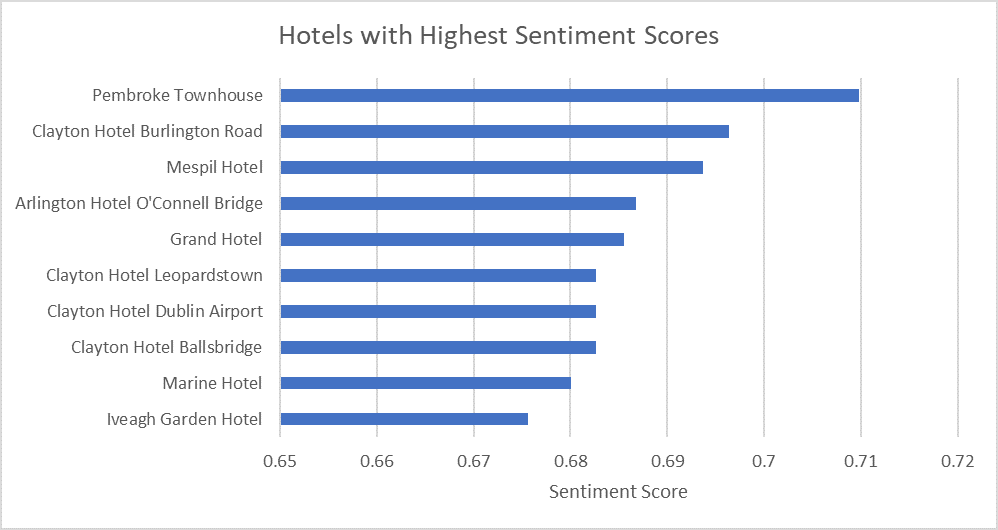
\includegraphics[width=0.95\textwidth]{evaluation/highest.png}
\caption{\label{fig:highest} Hotels with Highest Sentiment Scores.}
\end{figure}

\begin{figure}[h!]
\centering
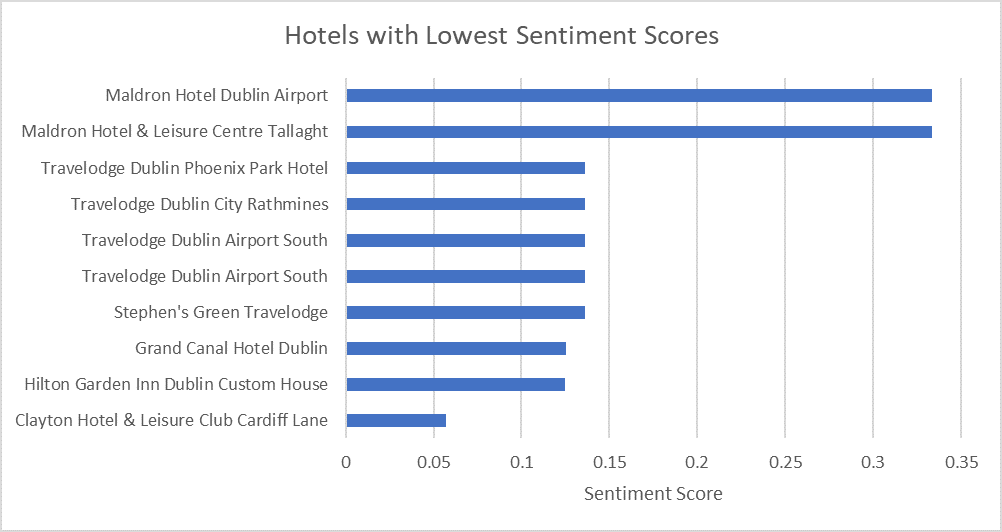
\includegraphics[width=0.95\textwidth]{evaluation/lowest.png}
\caption{\label{fig:lowest} Hotels with Lowest Sentiment Scores.}
\end{figure}

\section{Evaluation Metrics for Recommender Systems}

\subsection{Leave-One-Out Cross Validation}

The 'leave-one-out' cross validation approach involves removing one of a users n hotel bookings and using their remaining hotel bookings to generate the hotel recommendations. A list of hotels ranked in descending order by their predicted value is produced. The booking that was removed is compared to this list to see where it ranked, the higher the better. This is repeated with each of the users n bookings.

The 'leave-one-out' approach was used because of the data that we have. We do not have any explicit user reactions to recommendations but we do have implicit feedback in the form of user bookings. 

\subsection{Mean Percentile Rank}

The Mean Percentile Rank (MPR) is calculated based on the rankings recorded through leave-one-out cross validation. MPR is a recall-based measure. It measures the user satisfaction of items in an ordered list. The MPR formula is as follows:

\begin{equation}
    MPR = \frac{ \sum_{u,i} r_{ui} \times rank_{ui} } {\sum_{u,i} r_{ui}}
\end{equation}

$rank_{ui}$ is the percentile-ranking of hotel i within the ordered list of all hotels ranked for user u. $r_{ui}$ is a binary variable indicating whether user u booked hotel i. $rank_{ui} = 100\%$ indicates that the hotel i is predicted to be less desirable for user u. $rank_{ui} = 0\%$ indicates that the hotel i is predicted to be the most desirable hotel for user u. $rank_{ui} = 50\%$ would be expected for a list of randomly ranked hotels.

\section{Evaluation of Added Sentiment Scores}

\subsection{User Data}
The same Ryanair data that was used in the CoRE paper was used for evaluating each of the recommender systems. The Ryanair dataset consists of 29,704 hotel bookings, 11,638 unique hotels that have a least 1 booking and 20,223 users who made a booking at one or more hotels.

This project focused on hotels in Dublin so the dataset had to be filtered. The dataset was first filtered so that it only contained users with multiple hotel bookings. Multiple hotel bookings are required for the 'leave-one-out' approach so that a booking can be removed while still leaving at least one booking to use for generating the recommendations. Then the dataset was filtered so that it only contained users who had a booking in one of the Dublin hotels that we had produced a sentiment score for. The 'leave-one-out' approach had to be altered slightly so that the user's Dublin hotel booking was always the booking that was removed. The recommendations could be generated based on the other bookings but the removed booking had to be from Dublin so that we could evaluate where it ranked in the returned list.

There were 27 users who had multiple hotel bookings with at least one hotel booking in a Dublin hotel that we had a sentiment score for. The Dublin hotel bookings were for 21 different hotels. The evaluation was performed on these 27 users and 21 hotels. This is quite a small number of users which needs to be taken into consideration in the evaluation. Ideally we would like to evaluate the system on a much larger set of users and hotels, to verify our results. This is an area for future work.

\subsection{Baselines}

In order to assess the performance of SentiCoRE (CoRE with the added sentiment information) it was compared against multiple baselines. These included: 
\begin{enumerate}
    \item \textbf{Random} \newline
    A randomly ranked list of hotels.
    \item \textbf{Expedia Baseline} \newline
    The approach currently used by Ryanair in their rooms booking site. Hotels from the target city are sorted based on a sequence number given to them by Expedia. The sequence number is based on their transactional data from the last 30 days.
    \item \textbf{CoRE} \newline
    The CoRE recommender system without the sentiment score added in.
    \item \textbf{SentiCoRE} \newline
    The CoRE recommender system re-ranked with the sentiment scores produced by the Stanford NLP Sentiment Analyser.
\end{enumerate}

\section{Recommender Results and Analysis}

The results show that the addition of the sentiment score increases the MPR of CoRE, with and without feature weighting (Table ~\ref{Table:senticore}), which means the hotels are being ranked lower by SentiCoRE than CoRE. The best performing recommender system is CoRE. CoRE performs slightly better with feature weighting than without feature weighting as was seen in the evaluation of CoRE by itself \cite{core2019}. 

The Random Recommender which produces a random list of hotels performed the worst, which was expected. Typically a MPR of 50\% would be expected for a random list of hotels which is not far off the Random Recommender's MPR of 42.72\%. The Expedia Recommender only performed slightly better than the Random Recommender with a MPR of 40.87. Both CoRE and SentiCoRE performed significantly better than the Random and Expedia baselines.

\begin{table}[h!]
\setlength\extrarowheight{5pt}
\caption{Recommender Systems Performance.}
\label{Table:senticore}
\begin{tabular}{ll}
\specialrule{1.5pt}{1pt}{1pt}
\textbf{Recommender System} & \textbf{MPR (\%)} \\ \specialrule{1.5pt}{1pt}{1pt}
\rowcolor[HTML]{EFEFEF}
Random & 42.72 \\ \hline
Expedia Baseline & 40.87 \\ \hline
\rowcolor[HTML]{EFEFEF}
CoRE (with feature weighting) & 2.51 \\ \hline
CoRE (without feature weighting) & 3.31 \\ \hline
\rowcolor[HTML]{EFEFEF}
SentiCoRE (with feature weighting) & 14.68 \\ \hline
SentiCoRE (without feature weighting) & 9.92 \\ \hline
\end{tabular}
\end{table}

From the results, we can see that incorporating the sentiment scores into the CoRE recommender definitely has an impact on the hotel rankings. A positive sentiment score will move a hotel up the list while a negative ranking will move a hotel down the list. Taking only the MPR into account you would say that SentiCoRE is not performing as well as CoRE. However, SentiCoRE is having the desired effect and is adjusting the hotel rankings based on the sentiment scores.

\section{Summary}

One of the main aims of this research was to determine if it was possible to identify whether tweets contained reviews. A series of classifiers with different feature representations were implemented and evaluated. 

The best performing approach was a combination of the SVM Classifier and unigram TF-IDF feature representation, closely followed by bigram TF-IDF. 

The other aim of this research was to evaluate if review-like tweets could be used to appropriately influence the generation of recommendations in a recommender system. Sentiment scores were produced based on the classified tweets and used to re-rank the results of the CoRE recommender system. Incorporating the sentiment scores into the CoRE recommender had the desired effect and adjusted the rankings of the hotels. However, SentiCoRE performed worse than CoRE in terms of MPR.


\chapter{Conclusion}

\section{Summary of Results}

\section{Future Work}
One line of future work would be to improve the accuracy of the machine learning algorithms. This could be achieved by:
\begin{itemize}
    \item Increasing the size of the dataset. In general, supervised machine learning methods perform better on large datasets. This would involve gathering more tweets and manually annotating them.
    \item Investigating other feature representations. Part-of-speech tagging and natural language processing techniques could be experimented with.
    \item Trying more classification algorithms. Algorithms such as fakshfksj which were not evaluated in this research could be investigated. 
\end{itemize}

This research focused on hotels in Dublin. This scope could be expanded first geographically and then to different fields. Twitter could be used to gain sentiment information about restaurants, movies etc. and applied to recommender systems relating to these fields.

The Stanford NLP Sentiment Analyser was trained on a set of movie reviews from rotten tomatoes. It would be interesting to evaluate whether re-training the analyser using review-like tweets would improve it's performance. 

More data could be collected to evaluate the recommender system.

\section{Final Thoughts}
\bibliographystyle{unsrtnat}
\bibliography{bibs/dissertation_bibliography}
\appendix
\renewcommand{\thechapter}{A\arabic{chapter}}
\chapter{Appendix}

\begin{table}[h!]
\caption{Hotel Names and Twitter Handles.}
\label{Table:hotels}
\begin{tabular}{|p{7cm}|p{5cm}|}
\hline
\rowcolor[HTML]{EFEFEF}
\textbf{Hotel Name} & \textbf{Twitter Handle} \\ \hline
abberley hotel &  \\ \hline
abbey hotel &  \\ \hline
aberdeen lodge &  \\ \hline
academy plaza hotel & @academyplaza \\ \hline
accor hotels & @accorhotels \\ \hline
albany house & @albanyhouse \\ \hline
alex hotel & @thealexdublin \\ \hline
alexander hotel &  \\ \hline
ariel house & @arielhouse \\ \hline
arlington hotel & @arlingtondublin \\ \hline
ashling hotel & @ashlinghotel \\ \hline
aspect park west & @aspectparkwest \\ \hline
avoca house & @avocahouse \\ \hline
avondale house &  \\ \hline
baggot court townhouse &  \\ \hline
ballsbridge hotel & @bbhoteldublin \\ \hline
barrys hotel &  \\ \hline
beacon hotel & @thebeaconhotel \\ \hline
belvedere hotel & @belvederparnell \\ \hline
beresford hotel & @beresfordhoteli \\ \hline
blooms hotel & @bloomshotel \\ \hline
bonnington dublin &  \\ \hline
brooks hotel & @brookshoteld2 \\ \hline
buswells hotel & @buswellshotel \\ \hline
butlers townhouse & @butlersthd4 \\ \hline
camden court hotel & @camdencourt \\ \hline
carlton hotels & @carltonhotels \\ \hline
carnegie court & @carncourthotel \\ \hline
cassidys hotel & @cassidys\_hotel \\ \hline
castle hotel & @thecastlehotel \\ \hline
castleknock hotel & @cknock\_hotel \\ \hline
caulfields hotel &  \\ \hline
\end{tabular}
\end{table}


\begin{table}[h!]
\begin{tabular}{|p{7cm}|p{5cm}|}
\hline
\rowcolor[HTML]{EFEFEF}
\textbf{Hotel Name} & \textbf{Twitter Handle} \\ \hline
celtic lodge & @celticlodgedub \\ \hline
central inn &  \\ \hline
charleville lodge & @clodgehotel \\ \hline
city hotel &  \\ \hline
citywest hotel & @citywesthotel \\ \hline
clarence hotel & @theclarence \\ \hline
clarion hotel & @clarionnorden \\ \hline
clayton dublin airport & @claytoncarpark \\ \hline
clayton hotels & @claytonhotels \\ \hline
cliff townhouse & @clifftownhouse \\ \hline
clifton court hotel &  \\ \hline
clontarf castle & @clontarfcastle \\ \hline
cloverleaf suites & @cloverleafrs \\ \hline
clyde court hotel &  \\ \hline
conrad dublin & @conraddublin \\ \hline
croke park hotel & @crokeparkhotel \\ \hline
crowne plaza & @crowneplazablan \\ \hline
dawson hotel &  \\ \hline
dean dublin & @dean\_dublin \\ \hline
dergvale hotel &  \\ \hline
devlin dublin & @thedevlindublin \\ \hline
double tree & @doubletreedub \\ \hline
drury court hotel & @drurycourthotel \\ \hline
dublin city inn/dublin central inn & @dublincityinn \\ \hline
dylan hotel & @dylanhotel \\ \hline
ferryman townhouse &  \\ \hline
finnstown castle hotel & @finnstowndublin \\ \hline
fitzpatrick castle hotel & @fitzcastle \\ \hline
fitzsimons hotel &  \\ \hline
fitzwilliam hotel & @fitzwilliamdub \\ \hline
fleet street hotel & @fleetsthotel \\ \hline
gate hotel &  \\ \hline
generator hostel & @gen\_dublin \\ \hline
gibson hotel & @thegibsonhotel \\ \hline
glashaus hotel &  \\ \hline
gleann na smol &  \\ \hline
glen guesthouse &  \\ \hline
grafton capital &  \\ \hline
grafton guesthouse & @ghousedublin \\ \hline
grand canal hotel & @grandcanalhotel \\ \hline
grand hotel & @grandmalahide \\ \hline
green isle hotel & @greenislehotel \\ \hline
gresham hotel & @greshamhotel \\ \hline
\end{tabular}
\end{table}



\begin{table}[h!]
\begin{tabular}{|p{7cm}|p{5cm}|}
\hline
\rowcolor[HTML]{EFEFEF}
\textbf{Hotel Name} & \textbf{Twitter Handle} \\ \hline
hampton hotel & @hamptondublin \\ \hline
harcourt hotel &  \\ \hline
harding hotel &  \\ \hline
harrington hall &  \\ \hline
herbert park hotel & @herbertpark \\ \hline
hilton dublin & @hiltondub \\ \hline
hilton garden & @hgidublin \\ \hline
holiday inn & @hiexpress \\ \hline
hotel st. george by the key collection &  \\ \hline
house dublin 2 & @housedublin2 \\ \hline
intercontinental & @intercondublin \\ \hline
isaacs hostel & @isaacsdublin \\ \hline
iveagh garden & @iveaghgardenhot \\ \hline
jackson court & @jacksoncourtdub \\ \hline
jacobs inn & @jacobsinndublin \\ \hline
jurys inn & @jurysinnsdublin \\ \hline
key collection & @collectionkey \\ \hline
kildare street hotel &  \\ \hline
kingswood hotel citywest & @kingswooddublin \\ \hline
lansdowne hotel & @lansdownehotel1 \\ \hline
leeson inn downtown &  \\ \hline
louis fitzgerald & @louisfitzhotel \\ \hline
lynams hotel &  \\ \hline
maldron hotel parnell square &  \\ \hline
maldron hotels & @maldronhotels \\ \hline
maple hotel & @maplehotel \\ \hline
marine hotel & @marinehotel \\ \hline
marker hotel & @themarkerhotel \\ \hline
mercantile & @the\_mercantile \\ \hline
merrion hotel & @merrionhotel \\ \hline
mespil hotel & @mespilhotel \\ \hline
metro hotel & @metrohoteldub \\ \hline
metrostays &  \\ \hline
morehampton & @morehampton\_ \\ \hline
morgan hotel & @themorganhotel \\ \hline
morrison hotel & @morrisondublin \\ \hline
my place hotel & @myplacehotels \\ \hline
north star hotel & @northstar\_hotel \\ \hline
o'callaghan collection & @ochdublin \\ \hline
o'callaghan stephens green &  \\ \hline
o'shea's hotel & @hotelosheas \\ \hline
paramount hotel &  \\ \hline
parliament hotel & @paramounthotel \\ \hline
\end{tabular}
\end{table}


\begin{table}[h!]
\begin{tabular}{|p{7cm}|p{5cm}|}
\hline
\rowcolor[HTML]{EFEFEF}
\textbf{Hotel Name} & \textbf{Twitter Handle} \\ \hline
pembroke townhouse & @pembroketownhse \\ \hline
phoenix park hotel &  \\ \hline
plaza hotel & @plazatallaght \\ \hline
portobello hotel &  \\ \hline
premier suites & @premiersuiteseu \\ \hline
radisson blu & @radissondublin \\ \hline
ranelagh rooms & @ranelaghrooms \\ \hline
red cow moran hotel & @moranhotels \\ \hline
regency hotel &  \\ \hline
ripley court hotel &  \\ \hline
river house &  \\ \hline
roganstown hotel \& country club &  \\ \hline
roxford lodge & @roganstown \\ \hline
royal hotel and merrill leisure club & @royalhotelbray \\ \hline
royal marine & @royalmarine \\ \hline
russell court hotel &  \\ \hline
sandymount hotel & @sandymounthotel \\ \hline
schoolhouse hotel &  \\ \hline
shelbourne hotel & @theshelbourne \\ \hline
sheldon park hotel and leisure club & @sheldonpark\_ \\ \hline
sky backpackers &  \\ \hline
skylon hotel & @skylondublin \\ \hline
spencer hotel & @thespencerifsc \\ \hline
stauntons on the green & @stauntons\_ \\ \hline
staycity & @staycity \\ \hline
sweeney hotel &  \\ \hline
talbot hotel & @talbotstill \\ \hline
tara towers hotel & @taratowershotel \\ \hline
temple bar hotel & @templebarhotel \\ \hline
temple bar inn & @templebarinn \\ \hline
times hostels & @timeshostels \\ \hline
travelodge & @travelodge\_ire \\ \hline
travelodge dublin airport south &  \\ \hline
trinity city hotel & @trinity\_city \\ \hline
waterloo house &  \\ \hline
west county hotel & @westcountyhotel \\ \hline
westbury hotel & @westburydublin \\ \hline
westin dublin &  \\ \hline
white sands hotel & @whitesandshotel \\ \hline
wingate hibernian &  \\ \hline
wynn's hotel & @wynnshotel \\ \hline
\end{tabular}
\end{table}


\end{document}